%%%%%%%%%%%%%%%%%%%%%%%%%%%%%%%%%%%%%%%%%%%%%%%%%%%%%%%%%%%%%%%%%%%%%%%%%%%%%%%%
% TUM-Vorlage: Wissenschaftliche Arbeit
%%%%%%%%%%%%%%%%%%%%%%%%%%%%%%%%%%%%%%%%%%%%%%%%%%%%%%%%%%%%%%%%%%%%%%%%%%%%%%%%
%
% Rechteinhaber:
%     Technische Universität München
%     https://www.tum.de
% 
% Gestaltung:
%     ediundsepp Gestaltungsgesellschaft, München
%     http://www.ediundsepp.de
% 
% Technische Umsetzung:
%     eWorks GmbH, Frankfurt am Main
%     http://www.eworks.de
%
%%%%%%%%%%%%%%%%%%%%%%%%%%%%%%%%%%%%%%%%%%%%%%%%%%%%%%%%%%%%%%%%%%%%%%%%%%%%%%%%

%%%%%%%%%%%%%%%%%%%%%%%%%%%%%%%%%%%%%%%%%%%%%%%%%%%%%%%%%%%%%%%%%%%%%%%%%%%%%%%%
\documentclass[%
    fontsize=11pt, % Schriftgröße
    twoside=off % kein einseitiges Layout
]{scrbook} % Dokumentenklasse: KOMA-Script Book
\usepackage{scrlayer-scrpage} % Anpassbare Kopf- und Fußzeilen

\usepackage[utf8]{inputenc} % Textkodierung: UTF-8
\usepackage[T1]{fontenc} % Zeichensatzkodierung

%\usepackage[ngerman]{babel} % Deutsche Lokalisierung
\usepackage{graphicx} % Grafiken

% Schriftart Helvetica:
\usepackage[scaled]{helvet}
\renewcommand{\familydefault}{\sfdefault}

% Silbentrennung:
\usepackage{hyphenat}
\hyphenation{TUM in-te-res-siert} % Eigene Silbentrennung
%\tolerance 2414
%\hbadness 2414
%\emergencystretch 1.5em
%\hfuzz 0.3pt
%\widowpenalty=10000     % Hurenkinder
%\clubpenalty=10000      % Schusterjungen
%\vfuzz \hfuzz

\usepackage[hidelinks]{hyperref} % Hyperlinks
\usepackage[onehalfspacing]{setspace} % 1,5facher Zeilenabstand
\usepackage{calc} % Berechnungen
\usepackage{enumitem} % Mehr Kontrolle über itemize-, enumerate- und description-Umgebungen
\usepackage{relsize} % Schriftgröße in Abhängigkeit von aktueller anpassen
\usepackage{tabularx} % Flexiblere Tabellen
\usepackage{array}    % For new column types
\usepackage{booktabs}
\usepackage{multirow}
\usepackage[table]{xcolor} % For cell color

\usepackage[tablewithout, figurewithout]{caption} % Anpassen von Beschriftungen
\usepackage[colorinlistoftodos,prependcaption,textsize=tiny]{todonotes}
\usepackage{amsthm}
\usepackage{amssymb}
\usepackage{mathtools}
\usepackage{algorithmicx}
\usepackage{algorithm}     % For algorithm floating environment
\usepackage{algpseudocode} % For pseudocode styling
\algnewcommand{\FunctionName}[1]{\textproc{#1}}
\newtheorem{definition}{Definition}
\newtheorem{problem}{Problem}

% \def\wideentry#1#2{\begin{tabular}[t]{l}#1\\\hline#2\\#3\end{tabular}\linebreak[0]\ignorespaces}
\def\wideentry#1#2{\begin{tabular}[t]{l}\hline\textbf{#1}\\\hline#2 \\\hline\end{tabular}\linebreak[0]\ignorespaces}

\newcommand{\cfbox}[2]{%
    \colorlet{currentcolor}{.}%
    {\color{#1}%
    \fbox{\color{currentcolor}#2}}%
}


% Nummerierung von Abbildungen & Tabellen durchgängig, statt nach Kapiteln:
\usepackage{chngcntr}
\counterwithout{figure}{chapter}
\counterwithout{table}{chapter}

% Abkürzungen, Glossare:
\usepackage[%
    xindy,% xindy zum Indexieren verwenden
    acronym,% Separates Akronym-Verzeichnis
    nopostdot,% Kein Punkt am Ende einer Beschreibung im Glossar
]{glossaries}

% Spezielle Befehlsdefinitionen:
\newcommand{\Thema}{}

\usepackage{bookmark} % Lesezeichen

% Unterdrückung layoutbedingter Warnungen
\usepackage[immediate]{silence}
\WarningFilter[layout]{latex}{Reference `LastPage'} % Gesamtseitenzahl
\WarningFilter[layout]{lastpage}{Rerun to get the references right} % Gesamtseitenzahl
\WarningFilter[layout]{latex}{Label(s) may have changed.} % Referenz auf letzte Seite
\WarningFilter[layout]{textpos}{environment textblock* not in vertical mode} % Positionierung Seitenzahl
\WarningFilter[layout]{scrbook}{Change of } % Fußnoten-Trennzeichen im Text
\WarningFilter[layout]{tocbasic}{number width of} % Nummerbreite im Inhaltsverzeichnis
\WarningFilter[layout]{pdfTeX}{name{glo:abk} has been referenced but does not exist, replaced by a fixed one}

% My packages (Joao Olenscki)

% Debugging:
%\DeactivateWarningFilters[layout] % Unterdrückte Warnungen einschalten
%\usepackage{showframe} % Layout-Boxen anzeigen
%\usepackage{layout} % Layout-Informationen
%\usepackage{printlen} % Längenwerte ausgeben
 % !!! NICHT ENTFERNEN !!!

%%%%%%%%%%%%%%%%%%%%%%%%%%%%%%%%%%%%%%%%%%%%%%%%%%%%%%%%%%%%%%%%%%%%%%%%%%%%%%%%

\renewcommand{\Thema}{Improving spatio-temporal traffic prediction through transfer learning}

%%%%%%%%%%%%%%%%%%%%%%%%%%%%%%%%%%%%%%%%%%%%%%%%%%%%%%%%%%%%%%%%%%%%%%%%%%%%%%%%
\input{./resources/settings.tex} % !!! NICHT ENTFERNEN !!!
%%%%%%%%%%%%%%%%%%%%%%%%%%%%%%%%%%%%%%%%%%%%%%%%%%%%%%%%%%%%%%%%%%%%%%%%%%%%%%%%

\begin{document}

\title{Improving spatio-temporal traffic prediction through transfer learning}
\author{João Rodrigo Olenscki}
\date{07.02.2024}

%%%%%%%%%%%%%%%%%%%%%%%%%%%%%%%%%%%%%%%%%%%%%%%%%%%%%%%%%%%%%%%%%%%%%%%%%%%%%%%%

\chapter*{Abstract}

In urban planning and management, traffic prediction is essential for reducing congestion, optimizing urban layout, and estimating time throughout a city. Big data and \gls{AI} triggered a great leap forward in this field in recent years. Big data was a transformative concept in the field, changing how traffic data is collected, analyzed, and utilized. It allowed the collection of a significant volume of data with great diversity, a key enabler of \gls{AI} models, known for being data-greedy, as it optimizes data consumption, allowing these models to be computationally viable. 

State-of-the-art deep learning models can be highly accurate but require large amounts of data to work correctly. This drawback, called the ``cold-start'' problem, can prevent cities from building their intelligent network since inputting a certain amount of data is required to make the model functional. Recent studies have proposed the use of transfer learning mechanisms to handle this situation. These models can learn complex \gls{ST} patterns from data-rich cities and use this knowledge to make predictions in data-scarce counterparts. This kind of approach can also reduce the computational burden of re-training models, as the model developed to extract the complex patterns are reused even for other data-rich cities.

In this work, we delve into the study and adaption of state-of-the-art convolutional graph models into a transfer learning framework to take advantage of multiple cities as sources of knowledge on traffic patterns. For this purpose, we employed an extensive dataset with eight cities and studied the effects of different domain adaptation approaches and how, for instance, for a constant amount of source data, the diversity of origin of said data, using multiple source cities, affects the model's predictive ability. The baseline, with which we compared the models, comprised two statistical models: \gls{HA} and \gls{ARIMA}. To verify the accuracy of both the models and baselines, we employed several metrics, such as \gls{MAE}, \gls{RMSE},\gls{MSE}, and \gls{MAPE}.

The results found suggest that

\todo[inline]{complete abstract with results found}

%%%%%%%%%%%%%%%%%%%%%%%%%%%%%%%%%%%%%%%%%%%%%%%%%%%%%%%%%%%%%%%%%%%%%%%%%%%%%%%%


%%%%%%%%%%%%%%%%%%%%%%%%%%%%%%%%%%%%%%%%%%%%%%%%%%%%%%%%%%%%%%%%%%%%%%%%%%%%%%%%

\chapter*{Acknowledgments}

This thesis was written as part of my Master's degree in Mechanical Engineering at the Technical University of Munich at the Transporting Systems Engineering chair. First, I would like to express my gratitude to Univ.-Prof. Dr. Constantinos Antoniou and M. Sc. Cheng Lyu for allowing me to work on this project. They provided me with great counseling and discussions that helped a lot.

I want to express my gratitude to Univ.-Prof. Dr. Larissa Driemeier for serving as my co-supervisor in this thesis and to the Polytechnic School of the University of São Paulo for allowing me to study at TUM as part of a double degree program.

I also want to thank my friends with whom I discussed this thesis and from whom I found good listeners and advisors. In special, Lui, my companion during endless debugging sessions; Luís, João Pedro, and Ariel, my roommates and friends whom I used as rubber ducks, explaining problems and bugs in detail until I could figure out the causes; and Tomás, my dear brother with whom I could talk about the most various technical parts of this work in search of advice.

I am also very thankful to God for the strength, resilience, and courage during the writing of this thesis and for the entirety of my degree. To my parents, Ricardo and Camila, with whom I found support and love during this journey, this thesis is dedicated to you. I also thank all my siblings, José, Luís, Tomás, Sofia, Beatriz, and André, for their encouragement and help. I would also like to thank my uncle, aunt, and cousin, Hermann, Luciana, and Hermann, whose home was a second home for me during this year.

Finally, I thank everyone with whom I shared this part of my life, full of discoveries, a bit of hardship, and rich in personal growth. 


%%%%%%%%%%%%%%%%%%%%%%%%%%%%%%%%%%%%%%%%%%%%%%%%%%%%%%%%%%%%%%%%%%%%%%%%%%%%%%%%

\tableofcontents

\listoffigures

\listoftables

\listofalgorithms

\clearpage

\printglossary[type=\acronymtype,title=Glossary]

\clearpage

%%%%%%%%%%%%%%%%%%%%%%%%%%%%%%%%%%%%%%%%%%%%%%%%%%%%%%%%%%%%%%%%%%%%%%%%%%%%%%%%

\chapter{Introduction} \label{ch:intro}
\section{Motivation}

According to \cite{yin2015literature}, a \textit{smart city} can be defined as a well-coordinated system that integrates advanced technological infrastructure, relying on sophisticated data processing. The primary objectives of such integration are to enhance city governance efficiency, improve citizen satisfaction, foster business prosperity, and promote environmental sustainability. Within a smart city, the management of various individual systems that constitute the urban environment is not solely reliant on the data collected within the city; it also relies on different adaptable models that can learn and evolve to suit the specific needs and characteristics of the city. In this context, the development of traffic prediction models emerges as a pivotal component for establishing the foundational framework of smart city management.

Recent advances in deep learning, fed by the advent of Big Data, have led to significant advancements in prediction tasks related to traffic, such as crowd flow \cite{zhang2018predicting, jin2018spatio}, traffic flow \cite{polson2017deep, wu2018hybrid}, public transit flow \cite{liu2019deeppf, chai2018bike}, travel demands \cite{geng2019spatiotemporal}, and traffic speeds \cite{yu2017spatio}. While formidable in their predictive power, these models come with a substantial data appetite. This data requirement poses a challenge for initiating new intelligent networks because meaningful inferences remain elusive despite the considerable investment needed to establish the sensor network without access to substantial data history. This difficulty is known in the field as the ``cold-start'' problem.

To address the aforementioned challenge, novel techniques rooted in transfer learning  \cite{pan2009survey} have been introduced. These approaches enable training predictive traffic models for cities constrained by limited data by taking advantage of patterns observed in cities with abundant data resources. The fundamental concept behind these models involves the application of Multi-task Learning, a type of Inductive Transfer Learning, which entails initializing the network in the source city and implementing fine-tuning to adapt the network to the unique characteristics of the target city.

Additionally, the data representing the dynamic progression of urban traffic is inherently complex, encompassing two spatial dimensions and one temporal dimension. This multifaceted data is often expressed as a graph structure, where distinct segments or areas of the city are depicted as nodes, interconnected by unweighted edges constituting the physical connections between neighbor nodes. Effectively processing and interpreting this data necessitates specialized approaches. \gls{GCN} are generally employed for this purpose, adept at handling the intricacies of such graph-based representations.

Currently, state-of-the-art models don't focus much on leveraging diverse source data when generating domain-agnostic features in transfer learning frameworks. Some works consider the possibility of using multiple source cities in the domain adaptation process \cite{Yao2019, Lu2022, Tang2022}. Still, as of now, almost no paper delves into the impact diverse source domains can have on accuracy.

\section{Research Questions}

The main motivation of this thesis is to build a model capable of predicting the next state of a given traffic system. To reach this goal, the following objectives were drawn:

\begin{itemize}
	\item Analyze current state-of-the-art models and identify cells and architectures that could be used when building a novel model;
	\item Based on the results of the first objective, propose a novel model to be built, which should follow these requirements:
		\begin{itemize}
			\item capable of learning from multiple cities at the same time;
			\item capable of intra-city learning and
			\item capable of considering external features (such as weather data, \gls{POI} locations, relative date features).
			% \item capable of taking external data (such as weather data, \gls{POI} locations, holidays' calendar) as a supplement; and
			% \item with a pre-processing step that includes a data augmentation cell.
		\end{itemize}
	\item Analyze how impactful each feature derived from a requirement is to the model.
\end{itemize}

Concurrently, the following research questions were raised:

\begin{enumerate}[label=\textbf{Q.\arabic*}]
\item \label{q1} Is it possible to encompass more than two cities as sources in a transfer learning process?
\item \label{q2} What's the impact of the number of sources on the model's accuracy?
\item \label{q3} Is there a limit on the number of sources?
%\item \label{q4} Is data augmentation possible in the traffic prediction field?
\end{enumerate}

\section{Contribution}


\todo[inline]{contribution, ~2 paragraphs}


\section{Outline}

This work is organized as follows: Chapter \ref{ch:lit} introduces the literature review that was performed to further understand the problem and provides a comprehensive explanation of commonplace concepts of the field. Chapter \ref{ch:method} proposes a methodological framework for the entire work, including data acquisition, pre-processing, model building, and testing setup. Chapter \ref{ch:results} analyzes the results of the proposed tests and comparisons to proposed baselines. Chapter \ref{ch:discussion} uses the results to answer and discuss the research questions raised in Chapter \ref{ch:intro}. Chapter \ref{ch:conclusion} concludes the thesis and discusses the main directions for future research in the field.





\chapter{Literature Review} \label{ch:lit}
This chapter presents a literature review that we conducted to further the traffic forecasting field and its state-of-the-art.

\section{Traffic Forecasting} \label{sec:trafficforecasting}

Traffic Forecasting is a long-lasting field of study in Traffic Engineering, conceived in the 1950s \cite{Beckmann1956, Bevis1959}. Initially centered on traffic simulation, the area observed a significant upward trend in recent years. By its very nature, a traffic network constitutes a vast and complex system where events occurring at various junctures within the road grid can exert profound influence over the entire traffic flow. These inherent complexities render it an ideal subject for examination by cutting-edge machine-learning algorithms, such as \gls{LSTM}, \gls{GRU}, and \gls{CNN}.

Traffic network problems inherently comprise two domains: the temporal and spatial domains. In the early stages of deep learning model development for the field of traffic, a natural division emerged, allocating separate components to address each of these domains. For example, \gls{CNN} has conventionally been harnessed primarily for spatial feature extraction, which involves identifying elements' physical locations or arrangements within a given dataset. Conversely, \gls{RNN} has specialized in temporal feature extraction, focusing on discerning patterns that evolve or change over time.

The pioneering work of \cite{Ma2017} marked one of the earliest instances of employing \gls{CNN}s for traffic prediction tasks. Subsequently, this methodology proliferated across various model frameworks and underwent integration with other architectural paradigms. An illustrative example of this evolutionary trajectory emerges from the study conducted by \cite{Lin2021}, which employed a multiple \gls{GCN} framework. In this network type, the input to the convolutional layers consists of the city's graph representation.

Similarly, \cite{Zhao2017} was among the early proponents of employing \gls{LSTM} cells for short-term traffic prediction. This approach gained substantial traction, integrating cells into various models, as exemplified by the \gls{ConvLSTM} module introduced by \cite{yao2018deep}. In this architecture, spatial features were extracted at each time frame and subsequently fed into an \gls{LSTM} chain. This innovative approach allowed for the extraction of spatial and temporal features concurrently.

As a complex \gls{ST} problem, traffic forecasting offers a range of strategies, spanning from problem formulation to data structuring, encompassing data type selection. Regarding data representation, many authors \cite{Wang2019b, Yao2019, Wang20224695} choose to apply a grid in the city and treat each \mbox{1-by-1} region autonomously, computing variables (inflow and outflow, for instance) inside these boundaries. In this approach, the instantaneous snapshot of the city could be compared to an image in the context of image classification algorithms, with each pixel being equivalent to a region. 

An alternative to this structure is transforming the raw data, typically provided as a matrix or tensor, into a graph-based representation, with each geographical region converted into a distinct node and an adjacency matrix defining the connections between neighboring regions \cite{Ouyang20231, Jin2022731, Lin2021, Zhang2022, Geng2019, Wang2023, Lu2022, Tang2022, Wei2016}. This method can better capture the network's complexity and regions' nuanced connectivity. In contrast to the grid-based approach, where regions may share a border without necessarily sharing a connecting road, the graph representation effectively accounts for such subtleties.

A third strategy, applied in the works of  \cite{Elmi20201088, Li2022},  involves defining individual road segments as graph nodes. This approach offers significantly greater detail and precision in modeling traffic data as the data sources are condensed in a relatively small area. As a drawback, it also requires the installation of many more sensors to produce the data.



\section{Transfer Learning} \label{sec:transferlearning}

Transfer learning techniques \cite{pan2009survey} were introduced as valuable tools for addressing problems where existing knowledge or expertise from one domain could be employed to enhance learning and performance in another domain. These techniques prove incredibly beneficial when the latter domain suffers from a shortage of data. These techniques are widely used in \gls{NLP} problems such as sentiment and document classification. Furthermore, the computer vision field also benefited greatly from applying these approaches, as they are extensively used for image classification.

As many cities started to prepare themselves to transition into ``smart cities,'' they stumbled upon the ``cold start'' problem. This problem refers to the lack of data that a city faces after installing the sensor network and before acquiring enough data to justify deep learning models, and it is not unique to smart cities but resonates with the broader field of machine learning \cite{Ali2020}. In such a situation, managers must wait at least three months to make reasonable predictions with deep learning models despite all investments made in traffic prediction. In these cases, based on the assumption that despite being different, some cities can share a common behavior framework and have similar data distributions. Transfer learning favors acquiring knowledge from cities with abundant data and using this knowledge to understand and predict cities with scarce data.

Furthermore, Transfer Learning techniques are also suitable for intra-city transfer, i.e., transferring the learned patterns from a domain (for instance, bike sharing flow) to another in the same city (for example, pedestrian flow). This can observed in the work of \cite{Wang20224695}, in which the author used a taxi trip dataset to learn about bike sharing in the same city.

Generally, a transfer learning algorithm consists of three parts: feature extraction, in which \gls{ST} features are obtained through various ways; domain adaptation, in which the knowledge is transferred; and a predictor, responsible for making a prediction on the next step based on the extracted features obtained from the aforementioned parts.

The feature extraction step is also present in deep learning approaches to the traffic forecasting problem and it can be achieved by many different architectures, as discussed in Section \ref{sec:trafficforecasting}. On the other hand, the domain adaptation step is mainly present in the transfer learning networks and aims to extract transferable latent features between the domains. With it, one seeks to learn domain-invariant knowledge about the problem.

\subsection{Domain Adaptation}

On the efforts of domain adaptation, \cite{Wang20224695} proposes using convolutional layers parallelly for both source and target features. These convolutional layers are interconnected by calculating the \gls{MMD} between layers to form a transfer loss, which is then added to the overall model loss. \gls{MMD} is a statistical metric that quantifies the dissimilarity between two probability distributions  \cite{10.5555/2188385.2188410}. By using this metric as a loss function, the authors aimed to make the feature representation of different domains more similar. In like manner, \cite{Jin2022731} also proposes the use of \gls{MMD} to minimize the distance between features of different features and, in addition, the use of binary cross-entropy on the classification of the edge types, as the authors use multi-view graphs.

Despite working in a different field (network traffic prediction), \cite{Wang202222} uses a similar architecture to \cite{Wang20224695}, with the substitution of the \gls{MMD} cells for \gls{CTD} ones. With a similar loss calculation structure, the \gls{CTD} cells aim to measure the domains' discrepancy. \cite{Ouyang20231} explores a different approach. In their work, the authors propose using adversarial training for transfer learning. This implies the design of a discriminator and a predictor in the network to generate a transfer loss.

A different, more typical approach is used in \cite{Tang2022}, as the authors employ the parameter-sharing technique: pre-training on the source domain and fine-tuning on the target domain. In this technique, the parameters of the fine-tuning stage are initialized with the trained parameters from the pre-training phase. This adaptation is only possible when we assume that the difference between distinct domains is insignificant and that both domains may share common features and patterns.


In the same paper, \cite{Tang2022} also implements another knowledge transfer technique, the \gls{GRL}, proposed initially by \cite{ganin2015unsupervised}. This architecture features an identity forward pass and reverses the gradient signal during the backward pass. Considering that different cities possess unique spatial structures and compositions, the \gls{GRL} is designed to mitigate these discrepancies by fostering an adversarial training environment. This is achieved by reversing the gradient, which confuses the model during training and is coupled with a domain classifier. The domain classifier's task is to differentiate source and target domains. At the same time, the model, through the influence of the GRL, learns to generate domain-invariant features, thus enhancing its ability to generalize across different city datasets. This approach is convenient in scenarios where the goal is to adapt a model trained on one city's data (source domain) to perform accurately on data from another city (target domain) despite the inherent differences in their spatial characteristics.








% no TL -> 2, 13, 18, 19, 20


\chapter{Methodology} \label{ch:method}
In this chapter, we build a complete picture of the Methodology applied during the subject research. We briefly analyze the dataset used and describe all components of the implemented model and the training script used to generate the optimal weights for these components.

\section{Data Analysis and Exploration} \label{sec:data_analysis}

The dataset selected for sourcing the prediction model was part of the NeurIPS2021 Traffic4cast competition \cite{pmlr-v176-eichenberger22a}. This dataset consists of 360 days of data from 8 different cities with similar sizes derived from trajectories of a fleet of probe vehicles. The original data has 180 days from 2019 and another 180 days from 2020, as one of the questions of the challenge was to asses how the COVID pandemic affected traffic in different cities. As this represents a shift in the temporal distribution of the data, we choose not to use the 2020 half of it, intending to have an assumed temporal invariant distribution. Table\ref{tab:cities} disposes of all cities available on the dataset and the number of data points each city contains.

\begin{table}[!ht]
\centering
\begin{tabularx}{\textwidth}{ M | M | M }
\multicolumn{1}{X}{\textbf{City}}%
& \multicolumn{1}{X}{\textbf{\# of days}} 
& \multicolumn{1}{X}{\textbf{\# snapshots per day}}\\ \hline
Antwerp & 180 & 240 \\ \hline
Bangkok & 180 & 240 \\ \hline
Barcelona & 180 & 240 \\ \hline
Berlin & 180 & 240 \\ \hline
Chicago & 180 & 240 \\ \hline
Istanbul & 180 & 240 \\ \hline
Melbourne & 180 & 240 \\ \hline
Moscow & 180 & 240 
\end{tabularx}
\caption{List of the cities available on the dataset}
\label{tab:cities}
\end{table}

For a given time snapshot, the data of one city can be represented by a tensor of size $(495, 436, 8)$, where $495\times436$ represents the city grid, and $8$ stands for the channels, or pieces of information, per cell. These channels contain information on the volume and mean speed of the probe cars heading in the four diagonal directions. All data was normalized and discretized in the \texttt{uint8} range, meaning values are contained in the $[0, 255]$ range.

To better understand the data, distribution, and characteristics, the following analysis is conducted on the 5-minute snapshot that started at 12:00 on 9 January 2019 in Melbourne. Figures \ref{fig:speed} and \ref{fig:volume} show the distribution of values for both the speed (odd channels) and the volume (even channels). It's clear that while the volume has a more even distribution for non-zero values, there remains a massive bias for the zero values, as they represent more than 99\% of the data points. This indicates that most of our data comprises zeros and that activity should be treated as rare.

Furthermore, Figure \ref{fig:heatmap} confirms this theory, as it can be seen that most of the data for the speed channels is zero, and the volume, despite being better distributed, is also defined by a majority of zeros. Table \ref{tab:data_analysis} shows the statistics for each channel and reinforces the proposed thesis.



\begin{figure}[!ht]
    \centering
    \begin{minipage}{0.45\textwidth}
        \centering
        \includegraphics[width=0.9\textwidth]{./figures/speed.pdf}
         \caption{Histogram for data distribution for the speed. Note the first (very thin) bin with the null values.}
         \label{fig:speed}
    \end{minipage}\hfill
    \begin{minipage}{0.45\textwidth}
        \centering
        \includegraphics[width=0.9\textwidth]{./figures/volume.pdf}
         \caption{Histogram for data distribution for the volume. Note the first (very thin) bin with the null values.}
         \label{fig:volume}
    \end{minipage}
\end{figure}


\begin{figure}[!ht]
\noindent\hspace{0.5mm}\includegraphics[width=0.9\textwidth]{./figures/heatmaps_speed_volume.pdf}
\caption{Heatmap of the snapshot for the (a) Speed; and (b) Volume.}
\label{fig:heatmap}
\end{figure}


\begin{table}[!ht]
\centering
\begin{tabularx}{\textwidth}{ M | M | M | M | M }
\multicolumn{1}{X}{\textbf{Channel}}%
& \multicolumn{1}{X}{\textbf{Mean}} 
& \multicolumn{1}{X}{\textbf{Median}}
&\multicolumn{1}{X}{\textbf{Standard Deviation}}
&\multicolumn{1}{X}{\textbf{Non-zero elements}} \\ \hline
0 (volume) & 0.0216 & 0.0000 & 0.2861 & 1.08\% \\ \hline
2 (volume) & 0.0141 & 0.0000 & 0.2794 & 0.84\% \\ \hline
4 (volume) & 0.0133 & 0.0000 & 0.6236 & 0.72\% \\ \hline
6 (volume) & 0.0118 & 0.0000 & 0.5957 & 0.62\% \\ \hline
1 (speed)  & 0.6758 & 0.0000 & 9.5058 & 0.73\% \\ \hline
3 (speed)  & 0.8655 & 0.0000 & 11.3655 & 0.82\% \\ \hline
5 (speed)  & 0.7419 & 0.0000 & 10.5863 & 0.71\% \\ \hline
7 (speed)  & 0.6149 & 0.0000 & 9.8281 & 0.60\%
\end{tabularx}%
\caption{Statistics for each channel in the specific snapshot}
\label{tab:data_analysis}
\end{table}

\subsection{Data processing}

Some other data processing transformations were processed besides disposing of the 2020 half of the original data. A significant part of the motivation for this processing step is to reduce the input data's size (or shape) to make the models trainable in a reasonable time, given the limited computational resources available. The first one of the transformations implemented was the collapse of the even (volume) and odd (speed) channels by taking the mean of the data in every channel. Therefore, we were left with two channels: the volume and average speed of the cars in the particular region.


Furthermore, to allow efficient development of the model's components, only the central square of size $50\times 50$ was employed for the preliminary tests and experiments, including those used to tune the model's parameters. This may seem limiting at first glance, as it reduces the spatial coverage and may exclude potentially significant peripheral data. Nonetheless, this strategy is practically beneficial as it simplifies computational demands while capturing a substantial portion of traffic behaviors. The selected central area includes key urban sections characterized by informative traffic dynamics, which will help scale the model to encompass the entire urban layout.


%\begin{figure}[!ht]
%\noindent\hspace{0.5mm}\includegraphics[width=12cm]{./resources/Desert.jpg}
%\caption{Title, Author}
%\end{figure}


\section{Model Outline}

The proposed model consists of two modules: a Feature Extraction Network, modeled as the encoder of an autoencoder and explained in Section \ref{sec:fen}, and a Prediction Network, thoughtfully dissected in Section \ref{sec:pred}. Furthermore, Section \ref{sec:domainadap} is reserved for the exposition of the domain adaptation techniques employed through the model and during training to enable knowledge transfer between the domains. Section \ref{sec:training} summarizes with figures and pseudocode scripts how the model's training was done. This Section will explain the mathematical and formal basis for the model and the overall architecture to be built.


\todo[inline]{double check sections}

\subsection{Task}
The field of Spatio-Temporal prediction is vast, allowing researchers to try different approaches to problems that may seem the same. This can be observed from the bibliography presented in the bibliographic revision. It's essential to clearly define the problem to be solved and rigorously define the available information.

\begin{definition}\label{def:part}
A city $C$ is divided into a grid map of shape $W_{C}\times H_{C}$. Each partition $r_{i, j}$, with $1\leq i \leq W_C$ and $1\leq j \leq H_C$, is referred to as a region of $C$. The set containing all regions of the city is defined $R_C=\{r_{1, 1}, ..., r_{W_C, H_C}\}$.
\end{definition}

\begin{definition}\label{def:time}
The time range of available data of a city is divided into $T_{C}$  intervals of equal size: $t=[1, ..., t_{C}]$.
\end{definition}


\begin{definition}\label{def:ch}
For each region $r_{i, j}$, $N_{ch}$ data channels are available. These channels are the same for every city.
\end{definition}

By combining Definitions \ref{def:part}, \ref{def:time}, and \ref{def:ch} we can visualize the the 4D tensor of shape $(W_C, H_C, N_{ch}, T_C)$. Figure \ref{fig:data_tensor} shows a slice of this tensor. Each color represents a different channel, and each square of four colors represents a point in the 2D city grid. The stacked layers represent the time dimension.

\begin{definition} \label{def:dim}
A 4D tensor defines the data of a city $C$:
	\begin{equation}\label{eq:defdim}
		\mathcal{X}_C = \{x_{r, t}^{ch} | r \in R_C, t \in T_c, ch \in N_{ch}\}
	\end{equation}
\end{definition}

\begin{figure}[!ht]
\noindent\hspace{0.5mm}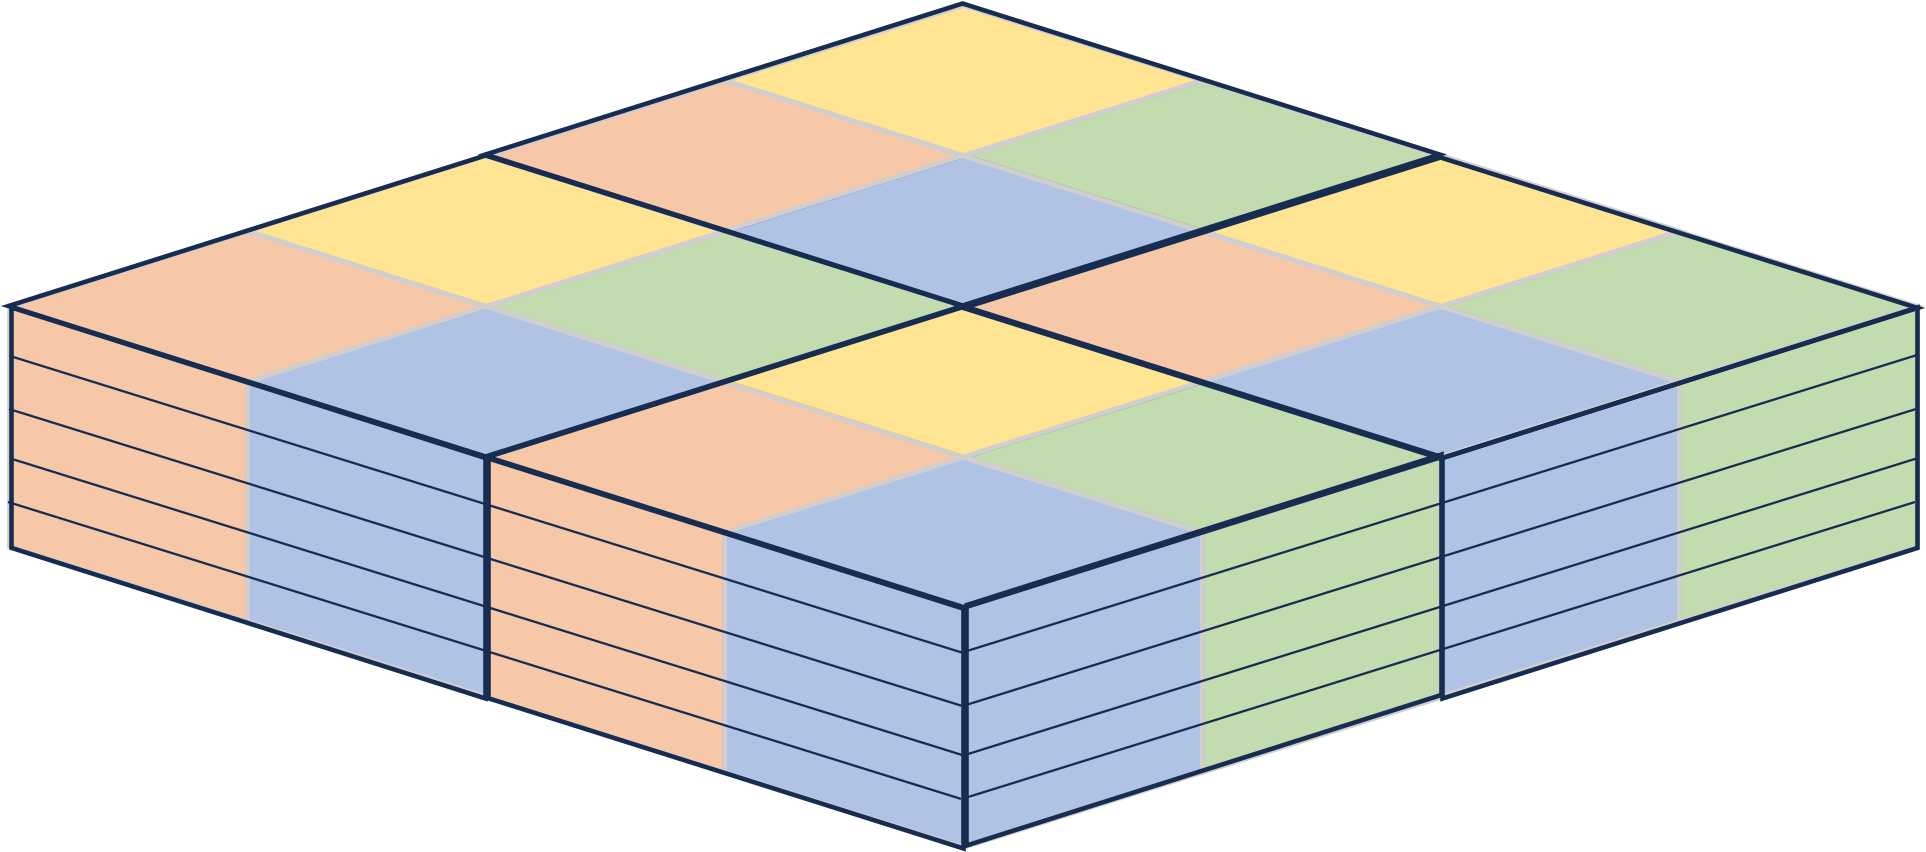
\includegraphics[width=0.6\textwidth]{./figures/data_tensor.pdf}
\caption{Visualization of the data (as a tensor).}
\label{fig:data_tensor}
\end{figure}

\begin{definition}\label{def:conn}
Connectivity in the city grid, denoted as \( \mathcal{E}_C \), is defined by the set of edges that establish the relationship between adjacent regions in \( C \). Each edge \( e_{k,l} \) in \( \mathcal{E}_C \) connects two regions \( r_{i,j} \) and \( r_{m,n} \), where \( i \) and \( m \) are indices within the width of the grid \( W_C \) and \( j \) and \( n \) are indices within the height of the grid \( H_C \). An edge exists if the regions it connects are adjacent horizontally, vertically, or diagonally, allowing for traffic data flow and convolutional operations across regions. Formally, the connectivity is represented as:
$$
\begin{aligned}
\mathcal{E}_C = \{ & e_{k,l} | e_{k,l} \text{ connects } r_{i,j} \text{ and } r_{m,n}, \text{ such that } |i - m| \leq 1 \text{ and } |j - n| \leq 1, \\
& \text{ for all } i, j, m, n \text{ that satisfy } 1 \leq i, m\leq W_C \text{ and } 1 \leq j, n \leq H_C \}
\end{aligned}
$$
\end{definition}


\begin{definition}\label{def:graph}
A graph representation of a city \( C \), denoted as \( G_C \), is defined as a tuple \( (V_C, \mathcal{E}_C,\mathcal{X}_C) \), where \( V_C \) is the set of nodes corresponding to the regions of \( C \), \( \mathcal{E}_C \) is the set of edges representing connectivity between regions, and \(\mathcal{X}_C \) is the node feature matrix, containing the feature (or channel) values of each node in \( V_C \). 
\end{definition}

Putting all previous definitions together, we define the adjacency matrix:

\begin{definition}\label{def:adj_matrix}
The adjacency matrix for a city \( C \), denoted as \( \mathbf{A}_C \), is a matrix that represents the connectivity between the nodes of \( C \) as defined in \( \mathcal{E}_C \) from Definition \ref{def:conn}. The adjacency matrix is a square matrix of size \( |V_C| \times |V_C| \), where \( |V_C| \) is the number of nodes in the graph representation of the city. Each element \( a_{ij} \) of the matrix \( \mathbf{A}_C \) is defined as follows:

$$
a_{ij} = 
\begin{cases}
1, & \text{if there exists an edge } e_{ij} \in \mathcal{E}_C \text{ connecting nodes } v_i \text{ and } v_j \\
0, & \text{otherwise}
\end{cases}
$$

This matrix is symmetrical, as the presence of an edge \( e_{ij} \) implies bidirectional connectivity between the nodes \( v_i \) and \( v_j \).
\end{definition}



With these definitions, it's possible then to define Problem \ref{prob:tl}:

\begin{problem} \label{prob:tl}
Given a data-scarce target city, $C_T$, and a set of $n$ data-rich source cities $\{C_{S1}, ..., C_{Sn}\}$, the problem proposed is to predict the value of the target city's data at $t_T+1$ with the historical data of the target city itself to that point and of the source cities:
	\begin{equation}\label{eq:probtl}
		\min_{\theta}\mathcal{L}(\tilde{\mathcal{X}}_{T, t_T + 1}, \mathcal{X}_{T, t_T + 1} )
	\end{equation}
	where
	\begin{equation}\label{eq:probtl2}
		\tilde{\mathcal{X}}_{T, t_T + 1} =  \theta(\mathcal{X}_{T, 1:t_T}, \{\mathcal{X}_{S1}, ..., \mathcal{X}_{Sn}\})
	\end{equation}
\end{problem}

Note that $ \mathcal{L}$ is the error criterion, which may vary depending on the data requirements. Note also that $t_{Sk} \gg t_T \forall k=1, ..., n$, indicating the target city's scarcity and the sources' richness.

\subsection{Proposed Architecture}

As explained at the beginning of this Section, the model comprises a Feature Extractor block modeled after the encoder of an autoencoder and a Predictor block. Figure \ref{fig:network_simplified} outlines the proposed architecture. Note that the individual modules will be developed and explained in their sections. The architecture adopted in this research draws upon the works of \cite{Wang202222, Wang20224695} as they proposed similar divisions in their models to transfer knowledge. Compared to their approach, we suggest using a \gls{STGAE} to train the feature extractor and an adjacency matrix to represent connectivity between the regions. Furthermore, the training part of the presented model is influenced by the work of \cite{Tang2022}, as we use similar domain adaptation techniques but delve into the influences that diversity on the source domain exerts on the model's accuracy.

\begin{figure}[!ht]
\noindent\hspace{0.5mm}\includegraphics[width=0.9\textwidth]{./figures/Model.pdf}
\caption{Simplified version of the proposed model.}
\label{fig:network_simplified}
\end{figure}

\section{Feature Extraction Network} \label{sec:fen}

As the first layer of the model, the Feature Extraction Network receives an input of tensors from one or more source cities and the target city and tries to extract, from these tensors, \gls{ST} features must be extracted to be used to train the Prediction Network. 

\subsection{Autoencoder}
 
Selecting hyperparameters and fine-tuning an extractor are challenging tasks in constructing a model, as it's difficult to observe causality between the change of a parameter and the change of the output due to the highly non-linear characteristics of these modules. As a result of these problems, the use of autoencoders for the feature extraction task has been proposed by \cite{Hinton2006}, and it's, as of today, a well-established paradigm in the \gls{ST} field. By conceptualizing the feature extraction process through the lens of an encoder, it becomes easier to verify its quality by constructing a corresponding decoder. As the encoder maps the input data from its original vectorial space to a latent space, the decoder pursues the contrary operation, returning the data from the latent space to the original one. In an ideal scenario, a well-trained autoencoder will reconstruct the original data perfectly, guaranteeing the quality of the features extracted by the encoder.
 
More recently, \cite{fan2023spatiotemporal} implemented a \gls{STAE} by coupling \gls{GLU} layers for time convolution and Chebyshev convolution layers for spatial convolution. By interpolating two temporal layers by a spatial one, the authors extracted both spatial and temporal features. Additionally, using Chebyshev filters of relatively large sizes ($K=6$), the proposed autoencoder could correctly derive features on both local and global scales.

In another paper, \cite{sabbaqi2022graph} proposes a generic framework for \gls{STGAE} with symmetric encoder-decoder architectures. The encoder finds a latent graph representation by applying graph convolutions, temporal downsampling layers, and activation functions. The decoder mirrors this behavior but uses temporal upsampling layers between the convolutions and activation functions. 
 
Figure \ref{fig:autoencoder} illustrates the architecture of the \gls{STGAE} utilized in our feature extraction framework. The encoder predominantly comprises a \gls{GConvLSTM} block for extracting spatio-temporal features. It is followed sequentially by an activation function, batch normalization, a regularization dropout layer, and a  linear transformation layer. Similarly, the decoder incorporates analogous components, adding a Sigmoid activation function preceding the output. This configuration leverages the data normalization previously applied, wherein the value range of all channels was linearly transformed from $[0, 255]$ to a unit interval $[0, 1]$.

\begin{figure}[!ht]
\noindent\hspace{0.5mm}\includegraphics[width=0.9\textwidth]{./figures/Autoencoder.pdf}
\caption{Diagram representing the autoencoder as a combination of an encoder and a decoder.}
\label{fig:autoencoder}
\end{figure}


\todo[inline]{verify if this diagram is up-to-date}

The \gls{GConvLSTM} cell, as implemented by \cite{rozemberczki2021pytorch}, and initially proposed by \cite{Seo_2018}, is parameterized by the number of input channels $N_{\text{in}}$, the number of output channels $N_{\text{out}}$, and the size of the Chebyshev polynomial filter $K$. The cell executes graph-based convolutions on the input tensor $x$, with the knowledge of the graph edge's descriptor tensor \texttt{edge\_index}, to yield the hidden state $h$ and the cell state $c$. These states are then propagated through the sequence for subsequent iterations, defined by the $k$ discrete temporal segments of which the input $x$ is composed. This enables the model to capture and encode the temporal dynamics of the data.

\begin{equation}
    \text{GConvLSTM}: \mathbb{R}^{D_1 \times D_2 \times \ldots \times D_N \times N_{\text{in}}} \rightarrow \mathbb{R}^{D_1 \times D_2 \times \ldots \times D_N \times N_{\text{out}}}
\end{equation}

Furthermore, as implemented in this layer, the order of the Chebyshev filter plays a pivotal role, as it defines the range of neighborhood aggregation. Specifically, it dictates how and how many local neighborhoods are expanded around each node during the convolutional process. This, in turn, influences the gradient computation during backpropagation, affecting both the receptive field and the capacity of the model to capture and integrate multi-hop relational information.

In a regular \gls{LSTM} implementation, all internal variables are calculated based on the sigmoid of combinations of fully connected layers as highlighted in the equations:

$$
\begin{aligned}
i_t & =\sigma\left(\boxed{W_{x i} x_t} + \boxed{W_{h i} h_{t-1}} + w_{c i} \odot c_{t-1}+b_i\right), \\
f_t & =\sigma\left(\boxed{W_{x f} x_t} + \boxed{W_{h f} h_{t-1}} + w_{c f} \odot c_{t-1}+b_f\right), \\
c_t & =f_t \odot c_{t-1}+i_t \odot \tanh \left(\boxed{W_{x c} x_t}+\boxed{W_{h c} h_{t-1}}+b_c\right), \\
o_t & =\sigma\left(\boxed{W_{x o} x_t} + \boxed{W_{h o} h_{t-1}} + w_{c o} \odot c_t+b_o\right), \\
h_t & =o \odot \tanh \left(c_t\right),
\end{aligned}
$$

Generalizing the \gls{LSTM}, a model developed for time-series forecasting, for graph inputs requires the adjustment of these operations for something that can handle graph-data input. For the \gls{GConvLSTM}, the authors implemented the graph convolution operator $\ast_\mathcal{G}$ proposed by \cite{cnn_graph}, in which a graph signal $x \in \mathbb{R}^{n}$ with $n$ nodes is filtered by a non-parametric kernel $g_\theta$ composed of vectors of Fourier coefficients.

\begin{equation*}
y = g_\theta \ast_\mathcal{G} x
\end{equation*}

On this implementation, $\ast_\mathcal{G}$ is modeled with the normalized graph Laplacian decomposition $L=U \Lambda U^T$, which would imply a model's complexity of $\mathcal{O}(n^2)$. To make it more feasible, the authors propose a truncated expansion of $g_\theta$ using Chebyshev polynomials $T_k$ and truncated laplacian $\tilde{L}$. This reduces the complexity to $\mathcal{O}(|\epsilon|n)$, with $\epsilon$ number of edges of the graph.

\begin{equation*}
y = g_\theta \ast_\mathcal{G} x = \sum_{k=0}^{K-1}\theta_k T_k(\tilde{L})x
\end{equation*}

Finally, it's possible to define the \gls{GConvLSTM} model.

\begin{equation}
\begin{aligned}
i & =\sigma\left(W_{x i}\ast_\mathcal{G} x_t+W_{h i}\ast_\mathcal{G} h_{t-1}+w_{c i} \odot c_{t-1}+b_i\right), \\
f & =\sigma\left(W_{x f}\ast_\mathcal{G} x_t+W_{h f}\ast_\mathcal{G} h_{t-1}+w_{c f} \odot c_{t-1}+b_f\right), \\
c_t & =f_t \odot c_{t-1}+i_t \odot \tanh \left(W_{x c}\ast_\mathcal{G} x_t+W_{h c}\ast_\mathcal{G} h_{t-1}+b_c\right), \\
o & =\sigma\left(W_{x o}\ast_\mathcal{G} x_t+W_{h o} \ast_\mathcal{G}h_{t-1}+w_{c o} \odot c_t+b_o\right), \\
h_t & =o \odot \tanh \left(c_t\right),
\end{aligned}
\end{equation}

\subsection{Fine Tuning}

The autoencoder, the most computationally demanding part of the entire model, owes much of its complexity to the \gls{GConvLSTM} layers in both the encoder and decoder. These layers execute graph convolution operations, which can become computationally intensive for large graphs due to their quadratic complexity, $\mathcal{O}(n^2)$, where $n$ is the number of nodes in the graph.

We suggest a pragmatic two-step training approach for the feature extractor to handle the computational demand more effectively. Initially, we train the autoencoder using the available source data, which allows us to establish a solid initial data representation. Subsequently, we fine-tune this representation with the target data, adapting it to the specific characteristics of the target domain.

Moreover, this method results in a fixed feature extractor not tightly coupled to the overall model. This flexibility is particularly beneficial when considering the parameter definition of the latter parts of the model, meaning that we can then focus on training the Prediction Network without feeling the effects that the choice of the feature extractor's parameter has on the results.

\section{Domain Adaptation} \label{sec:domainadap}

As one of the main challenges of a transfer learning task, domain adaptation is the process of adapting a model trained on one or more source domains (where abundant data is available) to perform well on a different but related target domain (where data is limited or has other distribution characteristics). Various approaches can be taken to tackle this problem in the different contexts that appear during the development of the model.

We suggest using two domain adaptors for this model: parameter sharing and a \gls{GRL}. The parameter sharing, which would be applied during a fine-tuning process after a pre-training, makes sure to start the network, which matters, the one that predicts the target values with the suitable weights to make it possible for this network to work correctly despite the lack of data points.

The \gls{GRL}, on the other hand, aims to help the feature extractor to produce domain-invariant features, which will then be extremely useful for transferring knowledge between different domains by making the encoder less sensitive to the specific characteristics of the source domain, thereby enhancing its ability to perform well on the target one. It's to be placed just after the encoder block of the autoencoder and before the decoder.

The \gls{GRL} is also used as part of an adversarial training strategy performed by a domain discriminator or classifier that tries to distinguish source and target domains. Since the \gls{GRL} reverses the gradient sign and scales it during backpropagation, it encourages the model to generate features that try to ``fool'' the domain classifier, which raises the loss but enforces the encoder to generate features that are domain-agnostic.

For the Domain Discriminator, we model it as a sequence of three operations: firstly, we apply a global mean pool to the features' tensor, followed by a linear layer, and then the softmax function. This will yield the probabilities that the features come from each domain (in this case, we have only two: source and target). With these probabilities, it's then possible to calculate a loss measure using \gls{BCE} loss. Figure \ref{fig:DomainDiscriminator} shows how this would look like and at which points of the overall model both the \gls{GRL} and Domain Discriminator would be placed.

In the Domain Discriminator block, a sequence of operations is designed to process the graph features effectively. Initially, a Top-K Pooling operation is employed to reduce the node count over all the graphs, selecting the $K_\text{pool}$ nodes with the most significant features from the last temporal segment output of the encoder. This process is essential for maintaining a consistent input shape for subsequent layers, ensuring the discriminator can operate uniformly on graphs from varying domains. After pooling, the features undergo batch normalization and dropout. The following linear layer projects the normalized and subsampled features onto a latent space, which a sigmoid function then squeezes into the $[0, 1]$ interval.

This operation translates the latent representations into probabilities, indicating the likelihood of the graph belonging to the target or source domain. These probabilities form the basis for computing the Domain Adversarial Loss with the \gls{BCE} Loss function. Figure \ref{fig:DomainDiscriminator} illustrates the placement of the \gls{GRL} and the Domain Discriminator within the overall model structure.


\begin{figure}[!ht]
\noindent\hspace{0.5mm}\includegraphics[width=0.9\textwidth]{./figures/DomainDiscriminator.pdf}
\caption{Diagram representing the architecture for the Domain Discriminator module.}
\label{fig:DomainDiscriminator}
\end{figure}


Given the output of the encoder block $H \in \mathbb{R}^{k\times N\times D_{lin}}$, with $k$ being the number of discrete temporal segments of which the input was composed, $N$ being the batched number of nodes of the input, and $D_{lin}$ the tunable dimension of the output of the linear layer of the encoder, we first select the last temporal segment from $H$. This choice is predicated on the understanding that the final snapshot encapsulates the most refined representation of the input graph, having undergone the full extent of recurrent processing through the \gls{LSTM} layers.

The next step in the pipeline is to apply the Top-K Pool to the graph. This is crucial in harmonizing node dimensionality across graphs from varied domains, which inherently may have disparate nodes. This step is essential to standardize the input size for the domain discriminator, allowing it to consistently and fairly assess the domain characteristics regardless of the original graph size. By retaining only the top $K_\text{pool}$ most significant nodes as per their learned representation in the encoder, Top-K Pooling concentrates on the most informative parts of the graphs, ensuring that the most critical structural and feature information is preserved for accurate domain discrimination.

\begin{equation}
	\text{Top-K Pool}:  \mathbb{R}^{N\times D_{lin}} \rightarrow \mathbb{R}^{K_\text{pool} \times D_{lin}}
\end{equation}

Following the dimensionality reduction via Top-K Pooling, the processed graph features are channeled through a linear layer, which projects the features onto a scalar. The subsequent application of the sigmoid function maps these projections to a $[0, 1]$ range, with the output values near 0 or 1 interpreted as the probability of the graph belonging to the target or source domain, respectively. These probabilities are then used to determine the Domain Adversarial Loss using the \gls{BCE} function - which will be presented and explained in Section \ref{ssec:bce}.

The general loss for the autoencoder training will then be defined accordingly to Equation \ref{eq:loss_ae}, with $\lambda$ being a tunable regularization parameter for balancing both the reconstruction loss $\mathcal{L}_{\text{feat}}$ and this adversarial loss $\mathcal{L}_{\text{DAN}}$.

\begin{equation} \label{eq:loss_ae}
	\mathcal{L}_{\text{AE}} = \mathcal{L}_{\text{feat}} + \lambda \cdot \mathcal{L}_{\text{DAN}}
\end{equation}


\section{Prediction Network} \label{sec:pred}

The second and final part of the model is the Prediction Network, which is responsible for making the next step prediction on the system state based on the features generated by the feature extractor and contextual timestamp features (time-of-the-day and day-of-the-week).


Given that the autoencoder developed is sufficiently good and can recreate the original input tensor $x$ with high accuracy, it's possible to consider that the encoder has appropriately learned how to extract the relevant features from the input. Based on that assumption, we extract the encoder from the trained autoencoder and use it as the feature extractor. Note that for feature extraction, we would only require the encoder block of the autoencoder, as the decoder and the domain discriminator blocks are only helpful tools for training the encoder.

Figure \ref{fig:Predictor} exposes the proposed architecture for the predictor block. It comprises an attention graph convolution block, an activation function, a linear layer, and a sigmoid normalization.

\begin{figure}[!ht]
\noindent\hspace{0.5mm}\includegraphics[width=0.9\textwidth]{./figures/Predictor.pdf}
\caption{Diagram representing the architecture for the Predictor network.}
\label{fig:Predictor}
\end{figure}

The tensor $H$ is the aforementioned output of the encoder block, while the tensor $T$ is the tensor that encapsulates periodic relative time features within our dataset. These features are derived from a sine-cosine transformation to exploit the inherent cycles in traffic flow, such as the daily rush hour peaks or the variation in traffic between weekdays and weekends. For the hour-of-the-day, we calculate:

\begin{equation}
\begin{aligned}
	hour\_sin=\sin\left(2\pi \cdot\frac{current\_hour}{hours\_in\_day} \right) & , & hour\_cos=\cos\left(2\pi \cdot\frac{current\_hour}{hours\_in\_day} \right)
\end{aligned}
\end{equation}

And for the day-of-the-week, we calculate:

\begin{equation}
\begin{aligned}
	day\_sin=\sin\left(2\pi \cdot\frac{current\_weekday}{days\_in\_week} \right) & , & day\_cos=\cos\left(2\pi \cdot\frac{current\_weekday}{days\_in\_week} \right)
\end{aligned}
\end{equation}

Concatenating these results, we create the tensor $T=[hour\_sin, hour\_cos, day\_sin, day\_cos]$, providing a continuous and differentiable representation of time. This tensor is fused with the regular \gls{ST} feature tensor, generating $H'$. For the fusion process, the tensor $T$ was extended (by repetition) to have all but the last dimension match the shape of $H$. The fusion technique applied to join them was a simple concatenation.

The leading actor of the Predictor block is the \gls{A3T-GCN} cell, proposed by \cite{abs-2006-11583} and implemented in the \textit{Pytorch Geometric Temporal} package \cite{rozemberczki2021pytorch}. It comprises two parts: first, a temporal convolution layer will generate $N_{t}$ hidden states $h$ for an input of $N_{t}$ temporal snapshots. These hidden states will then be the input of an attention model that will determine the context vector capable of understanding global variation trends, with which we can predict the system's future steps.



\section{Model Training} \label{sec:training}

After introducing all components of the model, it's opportune to explain, in detail, how exactly these components are supposed to be trained. Figure \ref{fig:training_script} shows the proposed training script for the whole model.

\begin{figure}[!ht]
\noindent\hspace{0.5mm}\includegraphics[width=0.9\textwidth]{./figures/training_script.pdf}
\caption{Diagram representing the training script and domain adaptation process.}
\label{fig:training_script}
\end{figure}

The training starts with pre-training the autoencoder and the domain discriminators using the source cities. As the decoder reconstructs the input, we can calculate a loss value composed of both a reconstruction criterion and an adversarial loss. After a determined number of epochs, the optimizer parameters are resettled, and the autoencoder is again trained with only the target city's data.

We freeze the autoencoder's weights for the second part and import the encoder block as the feature extractor. Again, the first step is to pre-train the predictor using the source cities' data and fine-tune it with the target city. For a more formal and structured explanation, Algorithm \ref{alg:ae} exposes the training process of the autoencoder with domain discriminator, while Algorithm \ref{alg:pred} does the same for the predictor block.

Since we use batch normalization as a regularization technique for all parts of our model, we selected \textproc{AdamW} \cite{abs-1711-05101}, a variation of \textproc{Adam}, as the optimizer algorithm. This makes sense because \textproc{AdamW} applies weight decay in a manner that is more compatible with batch normalization layers. Unlike the original \textproc{Adam} optimizer, which adjusts gradients directly and can undesirably impact batch normalization's scale and shift parameters, \textproc{AdamW} modifies the weights directly decoupled from the gradients, leading to more stable and consistent training dynamics.

Additionally, the utilization of \textproc{GradScaler} is noteworthy. This technique is employed to mitigate the underflow in gradient values during the backpropagation process, which occurs when the magnitudes of the gradients are so small that they are approximated to zero in the numerical precision being used. \textproc{GradScaler} addresses this issue by multiplying the loss value, from which gradients are derived, by a constant scaling factor. This operation increases the magnitudes of the gradients, preventing them from going to zero. After the backpropagation step, the gradients are then divided by the same scaling factor to restore their original magnitudes, preventing underflows without significantly impacting the performance.

Furthermore, it's interesting that we clarify the datasets used for each step of the training and evaluation of the model. During the pretraining phase, the autoencoder is trained on a combined dataset comprising both source and target data. This strategy facilitates the exposure of the domain discriminator to target features, which, in conjunction with the \gls{GRL}, orchestrates the adversarial training of the autoencoder. The datasets from the source domains are uniformly sized, while the smaller target domain dataset is iteratively cycled to align with the larger source datasets. Also, to make sure that the Domain Discriminator is trained in an unbiased way, for each \textproc{batch} from the dataloader, we randomly select one city and use only this selected city and the target city to train the \gls{DD}.

To enhance consistency, the pretraining of the predictor is also done on this same mixed dataset. The \textproc{optimizer\_params} for the different tasks are different and tuned based on the behavior of the loss of each task over the epochs, which are also task-specific parameters to be tuned depending on the learning capacity of each part of the model.

During the fine-tuning phase, we reset the optimizers using new, smaller learning rate and weight decay values and focused on the target dataset only. For the autoencoder, we still train both the \gls{GRL} and \gls{DD} to ensure that the model can adapt to the specific characteristics of the target domain while preserving the domain-invariant nature of the features. Since the fine-tuning dataset is smaller and the learning rate is reduced, we expect this to refine the model's performance on the target domain while maintaining its ability to generalize across domains. For this training phase, the target city dataset comprised, at a base case, 2 weeks' worth of data (meaning 3360 data points) extracted from the whole dataset via random split.

All testing on the predictor is done with a never-seen target data dataset. This dataset consisted of all non-used data of the target city. As in our setup, we had the same amount of data for all cities (6 months or 43\;200 data points). We used then ca. 40\;000 data points for the testing.

\begin{algorithm}
\caption{Autoencoder with Domain Discriminator Training Process }
\label{alg:ae}
\begin{algorithmic}[1]
\Require $AE\_params$, $DD\_params$, $num\_epochs$, $dataloaders$, $AE\_criterion$, $optimizer\_params$, $BATCH\_SIZE$, $lambda$
\Ensure Autoencoder $ae$, Domain Discriminator $dd$, Gradient Scaler $scaler$
\State \FunctionName{Encoder}, \FunctionName{Decoder} $ \gets$ \Call{Autoencoder}{$AE\_params$}
\State $dd \gets$ \Call{DomainDiscriminator}{$DD\_params$}
\State $scaler \gets$ \Call{GradScaler}{}
\State $optimizer \gets$ \Call{AdamW}{$\{ae, dd\}$, $optimizer\_params$}
\For{$epoch = 1$ \textbf{to} $num\_epochs$}
	\For{each $dataloader$ in $dataloaders$} \Comment{pre-training and fine-tuning dataloaders}
    \For{each $batch$ in $dataloader$}
        \State $total\_loss \gets 0$
        \For{each $data$ in $batch$}  \Comment{each batch can comprise $N$ different cities}
            \State $x, edge\_index, batch \gets data$
            \State $H \gets$ \Call{Encoder}{$x, edge\_index$}
	\State $H \gets$ \Call{GradientReversalLayer}{$H$}
            \State $dan\_loss \gets$ \Call{DomainDiscriminator}{$H, batch$}
            \State $x\_recons \gets$ \Call{Decoder}{$H, edge\_index$}
            \State $feat\_loss \gets AE\_criterion(x\_recons, x)$
            \State $loss \gets feat\_loss  + lambda \cdot dan\_loss$
            \State $total\_loss \gets total\_loss + loss$
        \EndFor
        \State \Call{Backward}{$scaler.scale(total\_loss)$}
        \State \Call{Step}{$optimizer$}
        \State \Call{Update}{$scaler$}
        \State $optimizer$.zero\_grad()
        \EndFor
    \EndFor
\EndFor
\end{algorithmic}
\end{algorithm}



\begin{algorithm}
\caption{Predictor Training Process}
\label{alg:pred}
\begin{algorithmic}[1]
\Require $PR\_params$, $num\_epochs$, $dataloaders$, $PR\_criterion$, $optimizer\_params$
\Ensure Predictor $pred$, Autoencoder $ae$
\State $pred \gets$ \Call{Predictor}{$PR\_params$}
\State  \FunctionName{Encoder} $ \gets$ \Call{Autoencoder}{\textit{pretrained}}\Comment{pre-trained and fine-tuned autoencoder}
\State $optimizer \gets$ \Call{AdamW}{$\{pred\}$, $optimizer\_params$}
\State $scaler \gets$ \Call{GradScaler}{}
\For{$epoch = 1$ \textbf{to} $num\_epochs$}
    \For{each $batch$ in $dataloaders$}
        \State $total\_loss \gets 0$
        \For{each $data$ in $batch$}
            \State $x, edge\_index, y, T\_features \gets data$
            \State $H \gets$ \Call{Encoder}{$x$, $edge\_index$}
            \State $H \gets$ \Call{FusionFeatures}{$H$, $T\_features$}
            \State $y\_hat \gets$ \Call{Predictor}{$H$, $edge\_index$, $batch$}
            \State $loss \gets$ \Call{PR\_Criterion}{$y$, $y\_hat$}
            \State $total\_loss \gets total\_loss + loss$
        \EndFor
        \State \Call{Backward}{$scaler.scale(total\_loss)$}
        \State \Call{Step}{$optimizer$}
        \State \Call{Update}{$scaler$}
        \State $optimizer$.zero\_grad()
    \EndFor
\EndFor
\Function{FusionFeatures}{$H$, $T$}
    \State $T \gets$ \Call{Extends}{$H$.shape}
    \State $H \gets H$ concatenated with $T$ along the feature dimension
    \State \Return $H$
\EndFunction
\end{algorithmic}
\end{algorithm}

\section{Loss Functions} \label{sec:loss_func}

In this Section, we define and explain the loss functions, also known as cost functions or criteria, that will be implemented or tested on the model or its parts. From the following criteria, \gls{MAE} and \gls{MAPE} are to be used exclusively as performance metrics. The purpose of listing and implementing a varied array of loss functions is to determine the best fit for our problem and data.

In this section, we define and elucidate the various loss functions, also recognized as cost functions or evaluation criteria, which are to be implemented or assessed within the model or its components. Among the specified criteria,\gls{MAE} and \gls{MAPE} will be exclusively utilized as performance metrics. Listing and implementing various loss functions is to determine the ones with the best training performance considering the problem and dataset.

\subsection{Mean Squared Error (MSE)}

As the most known and traditional loss function, \gls{MSE} is widely used in almost all fields of machine learning. In particular, it's one of traffic forecasting models' most ``standard'' loss functions as it focuses on minimizing significant errors.

\begin{equation}
\mathcal{L}(y, \hat{y}) = \frac{1}{N} \sum_{i=1}^{N} (y_i - \hat{y}_i)^2
\end{equation}


\subsection{Root Mean Squared Error (RMSE)}

A typical variation of the \gls{MSE}, \gls{RMSE} is widely used in almost all fields of machine learning for testing as a performance metric. It is based on the same concept that governs its base function but on the same scale as the input data. 

\begin{equation}
 \mathcal{L}(y, \hat{y}) = \frac{1}{N} \sqrt{\sum_{i=1}^{N} (y_i - \hat{y}_i)^2}
\end{equation}

\subsection{Mean Absolute Error (MAE)}

The \gls{MAE} is not supposed to be used as a criterion during the training phase, but rather, it's widely used as a performance metric for testing. It calculates the average absolute difference between the predicted and actual values. It treats all errors equally and is particularly robust when dealing with outliers.

\begin{equation}
\mathcal{L}(y, \hat{y}) = \frac{1}{N} \sum_{i=1}^{N} |y_i - \hat{y}_i|
\end{equation}

As it measures the average magnitude of errors in a set of predictions without considering their direction, the \gls{MAE} offers a scale-dependent interpretation of how far off the predictions are, on average, from the actual values.

\subsection{Mean Absolute Percentage Error (MAPE)}

Similarly, \gls{MAPE} is another performance metric to be applied during the testing phase. It uses the same logic as the \gls{MAE} but calculates the percentage error of the absolute difference between the predicted and actual values. It's used in the same context as MAE, but it's easier to interpret and practical when dealing with data represented in different scales.

\begin{equation}
\mathcal{L}(y, \hat{y}) = \frac{100\%}{N} \sum_{i=1}^{N} \left| \frac{y_i - \hat{y}_i}{y_i} \right|
\end{equation}

\subsection{Weighted Mean Squared Error (WMSE)}

As a variant of the MSE, the \gls{WMSE} amplifies the significance of errors in certain parts of the dataset by multiplying each error by a specific weight. It's helpful in scenarios where certain data points are more critical than others and should have more influence on the total loss. Mainly, it's applied to heavenly imbalanced datasets, as is the case for the data used in this work. This criterion is also known as Zero Inflation Loss when defining a weight for zero values.

\begin{equation}
\mathcal{L}(y, \hat{y}) = \frac{1}{N} \sum_{i=1}^{N} w \cdot (y_i - \hat{y}_i)^2
\end{equation}


\subsection{Mean Squared Logarithm Error (MSLE)}

This other variation of the MSE criterion consists of the mean of the squares of the logarithmic differences between the predicted and actual values. This criterion reduces the impact of significant errors on large true values. They are applied to problems where the target values have a wide range.

\begin{equation}
\mathcal{L}(y, \hat{y}) = \frac{1}{N} \sum_{i=1}^{N} (\log(y_i + 1) - \log(\hat{y}_i + 1))^2
\end{equation}

\subsection{Weighted Mean Squared Logarithm Error (WMSLE)}

The Weighted Mean Squared Logarithm Error (\gls{WMSLE}) is a sophisticated criterion that combines the aspects of the Mean Squared Logarithm Error (\gls{MSLE}) and the Weighted Mean Squared Error (\gls{WMSE}). It addresses the challenge of imbalanced datasets, focusing on penalizing the errors associated with non-zero targets more heavily.

This loss function is particularly adept at handling datasets where the prediction of non-zero values is more crucial than the prediction of zeros, which may be abundant but less informative. The \gls{WMSLE} is therefore especially useful when the cost of an error varies depending on the magnitude of the true value, such as in datasets with many zero entries but where accurate prediction of the non-zero values is paramount, which happens to be the case in our dataset (as discussed in Section \ref{sec:data_analysis}). The \gls{WMSLE} is defined as follows:

\begin{equation}
\mathcal{L}(y, \hat{y}) = \frac{1}{N} \sum_{i=1}^{N} w \cdot (\log(y_i + 1) - \log(\hat{y}_i + 1))^2
\end{equation}


\subsection{Custom Huber Loss}

The Custom Huber Loss combines the \gls{MSE} and \gls{MAE}. It's quadratic for small errors and linear for significant errors. We can also apply a Zero Inflation Loss for zero target values. It's advantageous when dealing with outliers and versatile as it can have the best of both criteria on the domains they are the best.

% Custom Huber Loss
\begin{equation}
\mathcal{L}_{\delta, w}(y, \hat{y}) = 
\begin{cases} 
\frac{1}{2} w \cdot (y_i - \hat{y}_i)^2 & \text{for } y =0, \\
\frac{1}{2} (y - \hat{y})^2 & \text{for } |y - \hat{y}| \leq \delta, \\
\delta \cdot (|y - \hat{y}| - \frac{1}{2} \delta) & \text{otherwise.}
\end{cases}
\end{equation}


\subsection{Log-Cosh Loss}

The Log-Cosh error is defined by the logarithm of the hyperbolic cosine of the difference between the prediction and actual values. It has a shape similar to the \gls{MSE} but is smoother and less sensitive to outliers. It's useful as it has the robustness of the \gls{MAE} while maintaining the smooth gradient of the \gls{MSE}. This loss function is differentiable, unlike \gls{MAE}.

% Log-Cosh Loss
\begin{equation}
\mathcal{L}(y, \hat{y}) = \frac{1}{N} \sum_{i=1}^{N} \log(\cosh(\hat{y}_i - y_i))
\end{equation}

\subsection{Binary Cross Entropy} \label{ssec:bce}

In the binary classification, the \gls{BCE} loss penalizes deviations from the actual labels by comparing the predicted probabilities against the ground truth, providing a robust gradient signal for model updates during training.

\begin{equation}
\mathcal{L}(y, \hat{y}) = -\frac{1}{N} \sum_{i=1}^{N} [y_{i} \log(\sigma(\hat{y}_{i})) + (1 - y_{i}) \log(1 - \sigma(\hat{y}_{i}))]
\end{equation}


\section{Baselines} \label{sec:baselines}

To better understand the performance achieved by the models elaborated, we propose using two different baselines: \gls{HA} and \gls{ARIMA}. In this Section, we explain each of the baselines, how they are calculated, and how they are applied to the dataset.

\subsection{Historical Average} \label{ssec:ha}

As one of the most common baselines in this field, \gls{HA} is based on the premise of temporal consistency, leveraging the average of data from corresponding time periods in the past—such as previous weeks—to forecast current traffic conditions.


\subsection{ARIMA} \label{ssec:arima}

As the other most famous and employed non-transfer baseline model, \gls{ARIMA} is a statistical time-series regression based on autoregressive (AR) and moving average (MA) components, which account for past values and errors, respectively, along with an integrated (I) element for differencing to induce stationarity \cite{1678242}.


\chapter{Results} \label{ch:results}
\section{Computational Specifications and Training Times} \label{sec:com_train}

This section specifies the computational hardware used during the development of the model. Here, we detail the machines employed during training and testing and the time each part of this process consumes. Table \ref{tab:hardware} shows the GPU models used and the training times for each dataset configuration and part of the model. The RTX 3070 was available on a personal computer, while the Tesla T4 and RTX 4090 were run as servers. The availability of the computational resources in the workspace determined the usage of different machines. Besides the time spent on training, the model's performance does not depend on the GPU. The headers ``Central Square'' and ``Whole City'' should be interpreted as the ``Time to train - (in minutes, per epoch per source city) in this dataset configuration''.


%\begin{table}[]
%\begin{tabular}{llllll}
%\multicolumn{1}{c}{}          & \multicolumn{1}{c}{}    & \multicolumn{2}{c}{\textbf{Central Square}}       & \multicolumn{2}{c}{\textbf{Whole city}} \\ \hline
%\multicolumn{1}{c|}{GPU Model} & \multicolumn{1}{c|}{VRAM (GB)} & \multicolumn{1}{l|}{AE} & \multicolumn{1}{l|}{PRED} & \multicolumn{1}{l|}{AE} & PRED \\ \hline
%\multicolumn{1}{l|}{RTX 3070} & \multicolumn{1}{l|}{8}  & \multicolumn{1}{l|}{}   & \multicolumn{1}{l|}{}   & \multicolumn{1}{l|}{}         &         \\ \hline
%\multicolumn{1}{l|}{Tesla T4} & \multicolumn{1}{l|}{16} & \multicolumn{1}{l|}{60} & \multicolumn{1}{l|}{30} & \multicolumn{1}{l|}{}         &         \\ \hline
%\multicolumn{1}{l|}{RTX 4090} & \multicolumn{1}{l|}{24} & \multicolumn{1}{l|}{}   & \multicolumn{1}{l|}{}   & \multicolumn{1}{l|}{}         &         \\ \hline
%\end{tabular}
%\caption{Hardware specifications and training times}
%\label{tab:hardware}
%\end{table}

\begin{table}[!ht]
\begin{tabularx}{\textwidth}{ M | M | M | M | M | M }
\multicolumn{1}{X}{\textbf{GPU Model}}%
& \multicolumn{1}{X}{\textbf{VRAM (GB)}} 
& \multicolumn{2}{X}{\textbf{Central Square}}
& \multicolumn{2}{X}{\textbf{Whole City}} \\ \cline{3-6}
\multicolumn{1}{X}{}
& \multicolumn{1}{X}{}
& \multicolumn{1}{X}{\textbf{AE}}
& \multicolumn{1}{|X|}{\textbf{PRED}}
& \multicolumn{1}{|X|}{\textbf{AE}}
& \multicolumn{1}{X}{\textbf{PRED}} \\ \hline
RTX 3070 & 8 & 150 & 75 & & \\ \hline
Tesla T4 & 16 & 60 & 30 & & \\ \hline
RTX 4090 & 24 & & & & 
\end{tabularx}
\caption{Hardware specifications and training times}
\label{tab:hardware}
\end{table}

As observed in the Table, the training process is very time-consuming, even for powerful graphic cards. This is why, for the preliminary experiments, we chose to use only the Central Square of each city.

% autoencoder pre-training: 1 hour/epoch*N_cities
% autoencoder fine-tuning: 4 minutes/epoch
% predictor pre-training: 30 minutes/epoch*N_cities
% predictor fine-tuning: 2 minutes/epoch

% results in ~1h40/epoch*N_cities for training the model
% (collapsed channels, reduced city)
% one could expect the ``price'' to be then 1h40*10(size multiplier)*4(channels multiplier)= 60 hours/epoch*N_cities to train a full model
% training with only two epochs, one city: 120 hours = 5 days
% training with only two epochs, two cities: 240 hours = 10 days

\section{Autoencoder Experiments}

This Section will present the experiments on the variation of the autoencoder's parameters. Experiments \ref{ssec:exp1} to \ref{ssec:exp5} are related to the hyperparameter search for the autoencoder, while \ref{ssec:exp6} presents the impacts that parameter sharing as a domain adaptation technique.

Table \ref{tab:params_ae} shows the parameters used for most experiments in this Section. Note that when a different value is used for a determined experiment, this value would be stated on a similar table in the experiment explanation.

\begin{table}[!ht]
\begin{tabularx}{\textwidth}{ M | M }
\multicolumn{1}{X}{\textbf{Parameter}}%
& \multicolumn{1}{X}{\textbf{Value}} \\ \hline
Batch size                                  &  32                            \\ \hline
Number of cities                         & 2                            \\ \hline
Epochs                                       & 2                            \\ \hline
Chebyshev polynomial degree  & 2                            \\ \hline
Convolution dimension              & 16                           \\ \hline
Linear dimension                       & 8                            \\ \hline
Activation function                   & ReLU                      \\ \hline
Dropout rate                            & 0.5                         \\ \hline
Loss criterion                            & ZeroInflationLoss($w=100$)
\end{tabularx}
\caption{Fixed parameters for the autoencoder experiments}
\label{tab:params_ae}
\end{table}


\subsection{Experiment 1: Impact of the Chebyshev polynomial degree parameter on the autoencoder's performance} \label{ssec:exp1}


The Chebyshev polynomial degree is one of the parameters of the \texttt{GConvLSTM} cell used as the backbone of the autoencoder. It dictates the receptive field of the model, as it limits the number of neighbors that will be used to structure a computational graph during backpropagation. For instance, for a value of $K_{\text{cheb}}=1$, the computational graph will have a depth of 1, and only the nodes individually will be part of it. A $K_{\text{cheb}}=2$ implies that the computational graphs will contain not only the nodes themselves but the immediate neighbors of each node.

In this experiment, we evaluated the autoencoder's performance with varying values of \( K_{\text{cheb}} \), ranging from 1 to 6, while maintaining all other parameters as specified in Table \ref{tab:params_ae}. Figure \ref{fig:exp01boxplot} illustrates the distributions of both \gls{MAE} and \gls{MSE} for the corresponding \( K_{\text{cheb}} \) values. The boxplots reveal a discernible trend where both \gls{MAE} and \gls{MSE} metrics decrease as \( K_{\text{cheb}} \) increases from 1 up to 3, indicative of improved performance. The median of \gls{MAE} reaches its minimum at \( K_{\text{cheb}} = 3 \), suggesting this is the optimal Chebyshev polynomial degree for capturing the \gls{ST} features within the dataset, given the current parameter configuration. However, for \( K_{\text{cheb}} \) values greater than 3, there is an observable increase in variance and a slight rise in error metrics, which may signal a risk of overfitting. 

\begin{figure}[!ht]
\noindent\hspace{0.5mm}\includegraphics[width=0.9\textwidth]{./figures/exp01/boxplot.pdf}
\caption{\gls{MAE} and \gls{MSE} for the autoencoder with different values of $K_{\text{cheb}}$}
\label{fig:exp01boxplot}
\end{figure}


\subsection{Experiment 2: Impact of the number of source cities on the autoencoder's performance} \label{ssec:exp2}


\begin{table}[!ht]
\begin{tabularx}{\textwidth}{ M | M }
\multicolumn{1}{X}{\textbf{Parameter}}%
& \multicolumn{1}{X}{\textbf{Value}} \\ \hline
Batch size                                  & 8                            \\ \hline
\end{tabularx}
\caption{Specific parameters for Experiment 2}
\label{tab:exp02}
\end{table}

Experiment 2 deals with the impact of the number of cities on the autoencoder's performance. The number of cities indicates the data available to the model and the diversity and complexity presented. Four different values for the number of cities were considered: 1, 2, 4, and 8. The fixed parameters of the experiment are presented in Tables \ref{tab:params_ae} and \ref{tab:exp02}, and Figure \ref{fig:exp02boxplot} shows the results obtained.

For training over just one city $(N_{cities}=1)$, we observe a relatively high median value for both \gls{MAE} and \gls{MSE}, with a wide \gls{IQR}, suggesting that the model lacks generalization capabilities compared to the other models. Introducing another city to the model $(N_{cities}=2)$ seems to result in a slighter better median for the \gls{MSE}, but at the cost of outliers and a significantly higher median value for the \gls{MAE}. 

When training over four $(N_{cities}=4)$ and eight $(N_{cities}=8)$ cities, the model seem to behave similarly. It's noticeably better than the previous models when comparing the median values for both metrics, indicating better performance and generalization capabilities. There are outliers at $(N_{cities}=8)$, which may indicate a limit on how much diversity can be inputted into the model while trying to increase generalization capabilities.

The overall trend suggests that incorporating data from more cities enables the model to learn more generalizable features across different domains, reducing the model's bias toward specific cities' traffic patterns. It's worth noting that increasing the number of cities also increases the computational cost of training the model. Therefore, using the $N_{cities}$ values near 4 seems more optimal.

\begin{figure}[!ht]
\noindent\hspace{0.5mm}\includegraphics[width=0.9\textwidth]{./figures/exp02/boxplot.pdf}
\caption{\gls{MAE} and \gls{MSE} for the autoencoder with different number of cities}
\label{fig:exp02boxplot}
\end{figure}

\subsection{Experiment 3: Impact of the activation function on the autoencoder's performance} \label{ssec:exp3}


\begin{table}[!ht]
\begin{tabularx}{\textwidth}{ M | M }
\multicolumn{1}{X}{\textbf{Parameter}}%
& \multicolumn{1}{X}{\textbf{Value}} \\ \hline
Chebyshev polynomial degree  & 3                            \\ \hline
\end{tabularx}
\caption{Specific parameters for Experiment 3}
\label{tab:exp03}
\end{table}

The choice of activation function within neural network layers substantially impacts the model's ability to capture and represent complex patterns within the data. This experiment examines how the activation function selection influences the autoencoder's performance. Three standard activation functions were considered: ReLU, Sigmoid, and Tanh.

For this analysis, we trained separate autoencoder models using each activation function while keeping all other parameters constant, as specified in Tables \ref{tab:params_ae} and \ref{tab:exp03}. Figure \ref{fig:exp03boxplot} presents the distributions of \gls{MAE} and \gls{MSE} across the different activation functions.

The boxplots indicate that the model with the ReLU activation function exhibits a slightly higher median \gls{MAE} than the other functions but also has a broader \gls{IQR}, suggesting less consistent predictions across different instances. On the other hand, the model utilizing the Sigmoid function shows a tighter \gls{IQR} in \gls{MAE}, indicating less variability in its predictions. However, its median \gls{MAE} is higher. Interestingly, the Tanh function yields the lowest median \gls{MAE}, suggesting it may be the most effective at capturing the underlying \gls{ST} patterns for this dataset and model configuration.


\begin{figure}[!ht]
\noindent\hspace{0.5mm}\includegraphics[width=0.9\textwidth]{./figures/exp03/boxplot.pdf}
\caption{\gls{MAE} and \gls{MSE} for the autoencoder with different activation functions.}
\label{fig:exp03boxplot}
\end{figure}


\subsection{Experiment 4: Impact of the criterion function on the autoencoder's performance} \label{ssec:exp4}


\begin{table}[!ht]
\begin{tabularx}{\textwidth}{ M | M }
\multicolumn{1}{X}{\textbf{Parameter}}%
& \multicolumn{1}{X}{\textbf{Value}} \\ \hline
Chebyshev polynomial degree  & 4                            \\ \hline
\end{tabularx}
\caption{Specific parameters for Experiment 4}
\label{tab:exp04}
\end{table}

Another interesting choice that can be made in the autoencoder training is the criterion function that yields the backpropagated loss. In this experiment, we analyze how different loss functions can influence the autoencoder's performance. All criteria used here were presented and explained in Section \ref{sec:loss_func}. All other parameters are exposed in Tables \ref{tab:params_ae} and \ref{tab:exp04}. The losses considered were:

\begin{itemize}
	\item \gls{MSE}
	\item \gls{WMSE} $(w=10)$
	\item \gls{WMSE} $(w=100)$
	\item \gls{MSLE}
	\item \gls{WMSLE} $(w=10)$
	\item \gls{WMSLE} $(w=100)$
	\item Log-Cosh Loss
	\item Focal Loss $(\alpha=0.25, \gamma=2)$
\end{itemize}

Figure \ref{fig:exp04boxplot} provides a comparative overview of the performance of these criteria on the autoencoder. From the plots, it is evident that both Focal Loss (with the input parameters) and Log-Cosh Loss are worse than their pairs, showing more considerable overall error (\gls{MAE} and \gls{MSE}) and \gls{IQR}, indicating that they are not fit for being used as criteria.

 The traditional \gls{MSE} provides a baseline for comparison, exhibiting a moderate spread in \gls{MAE} values. The \gls{MSLE} is designed to be less sensitive to significant errors by emphasizing the logarithmic difference between the predicted and actual values, which is evident in the lower median \gls{MAE} it achieves compared to \gls{MSE}.

A more nuanced approach is observed with both \gls{WMSE} and \gls{WMSLE}, where introducing a weight factor ($w$) aims to penalize errors differently based on their magnitude. Notably, for the \gls{WMSE}, as the weight increases from $w=1$ (\gls{MSE}) to $w=10$ to $w=100$, the spread and median of the \gls{MAE} decrease, suggesting a tighter grouping of errors around a lower central value. However, an increase in weight also introduces a higher variance in \gls{MSE}, as indicated by the presence of outliers, particularly for $w=100$. This implies that while \gls{WMSE} can potentially reduce the average error, it may also lead to more extreme errors in some instances. For the \gls{WMSLE} criterion, a similar result is observed, with the increase of $w$ being associated with a smaller \gls{IQR} but a higher median of the \gls{MAE}.

\begin{figure}[!ht]
\noindent\hspace{0.5mm}\includegraphics[width=0.9\textwidth]{./figures/exp04/boxplot.pdf}
\caption{\gls{MAE} and \gls{MSE} for the autoencoder with different criterion functions.}
\label{fig:exp04boxplot}
\end{figure}

\subsection{Experiment 5: Impact of the latent dimension's size the autoencoder's performance} \label{ssec:exp5}

\begin{table}[!ht]
\begin{tabularx}{\textwidth}{ M | M }
\multicolumn{1}{X}{\textbf{Parameter}}%
& \multicolumn{1}{X}{\textbf{Value}} \\ \hline
Chebyshev polynomial degree  & 4                            \\ \hline
Activation function                   & Tanh                      \\ \hline
\end{tabularx}
\caption{Specific parameters for Experiment 5}
\label{tab:exp05}
\end{table}

Experiment 5 focuses on the impact of inner (or latent) layer dimensions on the autoencoder's performance. For this purpose, several pairs of convolutional and linear dimensions were tested and are exposed in Tables \ref{tab:params_ae} and \ref{tab:exp05b}. Furthermore, Table \ref{tab:exp05} shows the fixed parameters for the experiment.

\begin{table}[!ht]
\begin{tabularx}{\textwidth}{ M | M }
\multicolumn{1}{X}{\textbf{Convolutional Dimension}}%
& \multicolumn{1}{X}{\textbf{Linear Dimension}} \\ \hline
8    & 2     \\ \hline
8    & 4    \\ \hline
8    & 8    \\ \hline
16  & 4    \\ \hline
16  & 8    \\ \hline
16  & 16  \\ \hline
32  & 8    \\ \hline
32  & 16
\end{tabularx}
\caption{Tested pairs of convolutional and linear dimensions.}
\label{tab:exp05b}
\end{table}

Analyzing Figure \ref{fig:exp05boxplot}, it's possible to note that the convolutional dimension is the most critical parameter between the two. Models with smaller convolutional dimensions ($\texttt{conv\_dim}=8$) tend to have higher \gls{MAE} and \gls{MSE} values, indicating a lower performance. This suggests that these models may not have enough complexity to capture the data's relevant \gls{ST} features.

Going up to $\texttt{conv\_dim}=16$, we can observe a significant reduction in both metrics. This points to a better extraction feature, enabling the autoencoder to capture more of the data's complexity. Finally, with $\texttt{conv\_dim}=32$, we note an increase of the median and extremes of the error, but a smaller \gls{IQR}, suggesting that we've reached a point where overfitting starts to take effect on the model.

Considering the values of the linear dimensions now, there's no clear trend that we can extract from the results, as an increase in it for low values of convolutional dimension led to more significant errors, but for other values, it made no difference. It's important to note that increasing convolutional and linear dimensions implies higher model complexity and, thus, higher computational cost for training it. For this reason, settling for pairs like $(16, 4)$ or $(16, 8)$ is the best option for balancing performance with cost.

\begin{figure}[!ht]
\noindent\hspace{0.5mm}\includegraphics[width=0.9\textwidth]{./figures/exp05/boxplot.pdf}
\caption{\gls{MAE} and \gls{MSE} for the autoencoder with different pairs of latent dimension values.}
\label{fig:exp05boxplot}
\end{figure}

\subsection{Experiment 6: Pretraining as a domain adaptation technique for the autoencoder} \label{ssec:exp6}

\begin{table}[!ht]
\begin{tabularx}{\textwidth}{ M | M }
\multicolumn{1}{X}{\textbf{Parameter}}%
& \multicolumn{1}{X}{\textbf{Value}} \\ \hline
Batch size                                  & 16                         \\ \hline
Number of cities                        &  1                            \\ \hline
Epochs                                       & 4                            \\ \hline
Chebyshev polynomial degree  & 4                            \\ \hline
Activation function                   & TanH                      \\ \hline
\end{tabularx}
\caption{Specific parameters for Experiment 6}
\label{tab:exp06}
\end{table}

Experiment 6 is the first attempt to apply a fine-tuning technique to transfer knowledge from one model to another. It consisted of training the model across three different setups: using solely the target city data (``Target Only''), pretraining with data from one source city followed by finetuning on the target city data (``Pretrained w/ 1 Source''), and pretraining with data from two source cities before finetuning on the target city data (``Pretrained w/ 2 Sources''). The results, illustrated in Figure \ref{fig:exp06boxplot}, underscore the benefits of transfer learning through pretraining.

The ``Target Only'' model shows the higher median and \gls{IQR} for both \gls{MAE} and \gls{MSE} when compared to the pre-trained ones. Conversely, both pre-trained setups significantly reduce both error metrics' median and \gls{IQR}. This suggests that the pre-training is an effective method for domain adaptation, as the model gets significantly better at generalizing and accurately predicting the \gls{ST} patterns. Furthermore, the image also indicates that having more cities can enhance this technique, as the diversity of data presented in the model increases its generalization capacity, making it more accurate.

\begin{figure}[!ht]
\noindent\hspace{0.5mm}\includegraphics[width=0.9\textwidth]{./figures/exp06/boxplot.pdf}
\caption{\gls{MAE} and \gls{MSE} for the autoencoders using different pre-training strategies.}
\label{fig:exp06boxplot}
\end{figure}


\section{Predictor Experiments}

Given then an autoencoder capable of effectively extracting the relevant \gls{ST} features, it's necessary now to define good hyperparameters for the predictor part of the model. Experiments .... investigate the optimization of the model by parameter variation, while Experiments ... deal with the knowledge transfer part.

Similarly to how we organized the previous Section, Table \ref{tab:params_pred} shows the fixed parameters for all predictor experiments. If a parameter from this table is to be changed, it will be clearly stated on the particular experiment's specific parameters table.

\begin{table}[!ht]
\begin{tabularx}{\textwidth}{ M | M | M }
\multicolumn{1}{X}{\textbf{Module}}
& \multicolumn{1}{X}{\textbf{Parameter}}%
& \multicolumn{1}{X}{\textbf{Value}} \\ \hline
both & Batch size                                  & 64                          \\ \hline
both & Epochs                                       &  2                           \\ \hline
both & Number of source cities             & 1                            \\ \hline
both & Weeks of target data                             & 2            \\ \hline
\gls{AE} & Chebyshev polynomial degree  & 3                            \\ \hline
\gls{AE} & Convolution dimension              & 16                          \\ \hline
\gls{AE} & Autoencoder Linear dimension  & 8                            \\ \hline
\gls{AE} & Activation function                   & TanH                      \\ \hline
\gls{AE} &  Dropout rate                            & 0.5                         \\ \hline
\gls{AE} & Loss criterion                            & \gls{MSE}              \\ \hline
\gls{AE} & $\lambda$ regularization           & 0.1              \\ \hline
\gls{PRED} & Activation function              & ReLU                      \\ \hline
\gls{PRED} & Loss criterion                       & \gls{MSE}              \\ \hline
\gls{PRED} & Top-K Pooling                       & 1750            \\ \hline
\gls{PRED} & Linear Dimension                  & 32              
\end{tabularx}
\caption{Fixed parameters for Predictor experiments}
\label{tab:params_pred}
\end{table}


\todo[inline]{complete this introduction}


\subsection{Experiment 7: Impact of the lambda regularization on the predictor} \label{ssec:exp7}


As we complete the development of the autoencoder, it's essential to address one of the main challenges of the proposed model: to generalize the knowledge obtained on the source domain to the new, different target domain. As presented in the Methodology section, we aim to learn how to extract domain-invariant features, which hold the key to a model's ability to perform well across varied domains without succumbing to domain-specific biases.

In this context, Experiment 7 was designed to investigate the impact of balancing the reconstruction loss of the autoencoder with the domain discriminator loss, modulated by a regularization parameter $\lambda$. This parameter regulates the trade-off between the fidelity of the reconstruction and the degree of domain invariance imposed by the \gls{DD}. Since we're introducing a regularization technique in the model's training, we expect that the individual performance of the autoencoder must pay for this enhanced performance on the generalization of the features, as we try to ``fool'' it during training.

The values of $\lambda$ tested range from $0$ to $1$, including $0.001, 0.005, 0.01, 0.1, 0.5,$ and $1$. A value of $0$ means no regularization from the domain discriminator and, therefore, no adversarial training, while a value of $1$ means that reconstruction and domain discriminator losses have the same weight when composing the total loss.

Figure \ref{fig:exp07boxplot} exposes the results obtained from training these models. The plot suggests that including the domain discriminator loss positively impacts the model's prediction ability as the performance for $\lambda=0$ is inferior to that for $\lambda \neq 0$. In particular, we can observe that for the \gls{MAE} boxes, there's an apparent decrease in both median and max values when going from $\lambda=0$ to $\lambda=0.001$ and then from $\lambda=0.001$ to $\lambda=0.005$, from which point it's hard to observe significant changes on the performances. However, one can verify that the number of outliers on the maximum size of the boxes seems to increase.

One possible explanation for the lack of changes observed from a certain point onwards is that as we reach a point of stabilization during training, the reconstruction loss starts to reach low values (in the order of $10^{-4}$). At the same time, we maintain the domain discriminator loss oscillating around 0.6 (the ideal expected value for it is $\ln{(2)}\simeq 0.693$, which occurs when the domain discriminator can't identify the domain due to the features being completely domain-agnostic). This means that the domain discriminator loss, supposed constant, will dominate the total loss almost constantly, and, for a determined threshold, there's no difference between $\lambda=0.5$ and $\lambda=1$ as they both result in a seemingly significant loss for the optimizer.

\begin{figure}[!ht]
\noindent\hspace{0.5mm}\includegraphics[width=0.9\textwidth]{./figures/exp07/boxplot.pdf}
\caption{\gls{MAE} and \gls{MSE} on the prediction using different values of $\lambda$.}
\label{fig:exp07boxplot}
\end{figure}

\subsection{Experiment 8: Impact of the linear layer dimension on the predictor} \label{ssec:exp8}

\begin{table}[!ht]
\begin{tabularx}{\textwidth}{ M | M | M }
\multicolumn{1}{X}{\textbf{Module}}
& \multicolumn{1}{X}{\textbf{Parameter}}%
& \multicolumn{1}{X}{\textbf{Value}} \\ \hline
\gls{PRED} & Activation function              & ReLU                      \\ \hline
\gls{PRED} & Loss criterion                       & \gls{MSE}              \\ \hline
\gls{PRED} & Top-K Pooling                       & 1750          
\end{tabularx}
\caption{Specific parameters for Experiment 8}
\label{tab:exp08}
\end{table}

Experiment 8 was projected to better understand the impact of the linear layer dimension, the output size of the \gls{A3T-GCN} layer, on the model's performance. The experiment assessed four sizes for the linear dimension: 8, 16, 32, and 64. Figure \ref{fig:exp08boxplot} shows the \gls{MAE} and \gls{MSE} distribution for the different compositions. With the increase in the size of the output of the convolutional block, the median of both metrics also increases, suggesting potential overfitting or a decrease in the model's ability to generalize.

\begin{figure}[!ht]
\noindent\hspace{0.5mm}\includegraphics[width=0.9\textwidth]{./figures/exp08/boxplot.pdf}
\caption{\gls{MAE} and \gls{MSE} on the prediction using different domain adaptation techniques.}
\label{fig:exp08boxplot}
\end{figure}

\subsection{Experiment 9: impact of the number of epochs on the predictor}

In machine learning terms, an epoch represents a complete cycle through the data, providing the model with repeated exposure to the training examples and allowing it to incrementally adjust its parameters. Changing the number of epochs to be used impacts the model's performance directly, as an epoch count that is too low may lead to underfitting. At the same time, too many epochs can cause overfitting. This investigation is critical for understanding the temporal dynamics of model convergence and identifying the most resource-efficient training regimen that maintains or enhances model efficacy.

For this experiment, we tested the model proposed using five different values of the number of epochs, ranging from 1 to 5, to be used on the autoencoder and predictor training. Figure \ref{fig:exp09boxplot} contains the results obtained. There's a clear trend of improvement in the model's performance as we increase the number of training epochs. We can observe a considerable gap on both \gls{MAE} and \gls{MSE} from one to two epochs. Still, the rate of improvement appears to diminish after that, as the median for the remaining boxes seems to share similar medians and \gls{IQR}. Nonetheless, we can observe that the maximum error (for both metrics) continues to decrease with the increase of epochs. This indicates that the model is becoming more robust to outliers and noise in the data.

As we reach three training epochs, we've got a plateau regarding median error for the metrics, suggesting that the model may be approaching its learning capacity given the provided data. As we're dealing with a relatively large training dataset (in both numbers of data points and information/nodes per data point), it's plausible to consider that with only three epochs, the model has effectively learned how to capture the underlying patterns in the data. Since, as discussed in Section \ref{sec:com_train}, an epoch of training with one source city takes approximately two hours, given the computational resources available, we can consider that the modest number of three epochs is sufficient for the model to learn. We can allocate the processing power into other areas of the model, such as supporting more source cities.

\begin{figure}[!ht]
\noindent\hspace{0.5mm}\includegraphics[width=0.9\textwidth]{./figures/exp09/boxplot.pdf}
\caption{\gls{MAE} and \gls{MSE} on the prediction using different number of epochs.}
\label{fig:exp09boxplot}
\end{figure}



\subsection{Experiment 10: Impact of the scarcity of the target dataset}

As the volume of available target data is one of the main grounds on which the development of transfer learning models is based, we find it interesting to experiment with how the availability of this kind of data impacts the overall performance of the model. By incrementally increasing the quantity of target data from 1 to 4 weeks, we aim to uncover how the breadth of target domain exposure affects the model's capacity to learn and generalize. Also, for many decision-makers, for which such models must yield important information that will govern their decisions, the availability of such data has a monetary price. By examining the model's performance with 1, 2, 3, and 4 weeks of target data, we can evaluate the prediction performance one can obtain for that price.



\section{Full Model Experiments}

Building upon the insights obtained from the previous experiments, we now assess the entire model, experimenting with the complete model in its best possible form. Also, to test the model in its best extension, for this Section, we use the entire city's data, not only the central square we've been using until now to save computation resources (as discussed in Section \ref{sec:data_analysis}).

Furthermore, for this section, the trained models will be tested against two baselines: \gls{ARIMA} and \gls{HA}, standard baselines in traffic prediction. All baselines and models are evaluated by three metrics: \gls{MAE}, \gls{MAPE}, and \gls{RMSE}.



\chapter{Discussion} \label{ch:discussion}
\section{On the hyperparameter search} \label{sec:hyperparam}

\section{On the model's performance} \label{sec:modelperf}

\section{Research Questions} \label{sec:research_answer}

\subsection{Q.1}



\subsection{Q.2}



\subsection{Q.3}




\chapter{Conclusion} \label{ch:conclusion}
This Chapter, as announced before, has the purpose of summarizing the thesis' key findings and outlining the contributions of the work presented here to the state-of-the-art of the traffic forecasting field, as well as showing the limitations we found during the development of these complex models and addressing the possible future path to take to overcome them. It's divided into two parts: Section \ref{sec:summary} reviews the entirety of the thesis, highlighting its main points and contributions. Section \ref{sec:limitations_future} exposes the limitations faced and sets the future directions to expand upon these findings.

\section{Summary and Contribution} \label{sec:summary}



\section{Limitations and Future Research} \label{sec:limitations_future}	




%\section{Section}
%
%\subsection[]{Subsection}
%
%Example of a figure, see below.
%
%\begin{figure}[!ht]
%\noindent\hspace{0.5mm}\includegraphics[width=12cm]{./resources/Desert.jpg}
%\caption{Title, Author}
%\end{figure}
%
%Example of glossary use: \gls{ITS}.
%
%Example use of citation \cite{Wang2023}.
%
%\clearpage
%
%\chapter{Tables}
%
%\vspace{\parskip}
%\section*{Table style 1}
%
%\begin{table}[!h]
%\begin{tabularx}{\textwidth}{ M | M }
%\multicolumn{1}{X}{\textbf{Spalte 1}}%
%& \multicolumn{1}{X}{\textbf{Spalte 2}} \\
%\hline
%Nummer 1 & Nummer 2 \\
%\hline
%Nummer 1 & Nummer 2 \\
%\hline
%Nummer 1 & Nummer 2 \\
%\hline
%\end{tabularx}
%
%\caption{Caption}
%\end{table}
%
%\vspace{\parskip}
%\section*{Table style 2}
%
%\begin{table}[!h]
%\begin{tabularx}{\textwidth}{| M | M |}
%\hline
%\textbf{Spalte 1} & \textbf{Spalte 2} \\
%\hline
%Nummer 1 & Nummer 2 \\
%\hline
%Nummer 1 & Nummer 2 \\
%\hline
%Nummer 1 & Nummer 2 \\
%\hline
%\end{tabularx}
%
%\caption{Caption}
%\end{table}
%
%\vspace{\parskip}
%\section*{Table style 3}
%
%\begin{table}[!h]
%\begin{tabularx}{\textwidth}{@{} M  M @{}}
%\textbf{Spalte 1} & \textbf{Spalte 2} \\
%Nummer 1 & Nummer 2 \\
%Nummer 1 & Nummer 2 \\
%Nummer 1 & Nummer 2 \\
%\end{tabularx}
%
%\caption{Caption}
%\end{table}

%%%%%%%%%%%%%%%%%%%%%%%%%%%%%%%%%%%%%%%%%%%%%%%%%%%%%%%%%%%%%%%%%%%%%%%%%%%%%%%%
\clearpage
%\nocite{*}
\bibliographystyle{ieeetr}
\bibliography{references}

\end{document}